%% UF thesis template from https://helpdesk.ufl.edu/application-support-center/etd-technical-support/ms-word-and-latex-templates/
%% LaTex template summer 2019

\documentclass{ufdissertation}\sloppy

\usepackage[T1]{fontenc}
%\usepackage[utf8]{inputenc} % seems it is by default and not needed
\usepackage{charter}

\usepackage{ragged2e} % to make text fully justified

\usepackage{tikz}%       tikz is used by almost everyone, but certainly by me for this.
\usepackage[compat=1.1.0]{tikz-feynman}% for drawing feynman diagrams 
\usepackage{pgfplots}%   pgfplots is tikz but better.
\usepackage{xspace}
\usepackage{xcolor}
\usepackage{caption}
\usepackage{subcaption} % allowing to use subfigure inside figure
\usepackage{topcapt} % allow \topcaption
\usepackage{graphicx} % allow \resizebox

%\usepackage{amsrefs}%   amsrefs contains the .bibtex style content for mathematician papers.
\usepackage{amsmath}


% Enable format for table, figure, object
\haveTablestrue%        Uncomment this if you have tables in your thesis.
\haveFigurestrue%       Uncomment this if you have figures in your thesis.
\haveObjectstrue%       Uncomment this if you have Objects in your thesis. This is almost certainly not the case however.


% Author info
\title{A Search For The Standard Model Higgs Boson Decaying Into Two Muons In The Vector Boson Associated Production Mode At The CMS Experiment}

\degreeType{Doctorate of Philosophy}%   Official name of your degree; eg "Doctorate of Philosophy".
\major{Physics}%                    Your official Department
\author{Xunwu Zuo}%                  Your Name
\thesisType{Dissertation}%              Dissertation (PhD) or Thesis (Masters)
\degreeYear{2021}%                      Intended graduation year (not the year you submit the thesis)
\degreeMonth{May}%                   Month of graduation should be May, August, or December.
\chair[Darin Acosta]%                   Chair and Cochair (see comment block above).

%% additional sections
%\setDedicationFile{dedicationFile}%                 Dedication Page
%\setAcknowledgementsFile{acknowledgementsFile}%     Acknowledgements Page
%\setAbstractFile{abstractFile}%                     Abstract Page (This should only include the abstract itself)
\setReferenceFile{referenceFile}{amsplain}%         References. First argument is your bibtex source file
%%                                                       the second argument is your bibtex style file.
%\setBiographicalFile{biographyFile}%                Biography file of the Author (you).
%
%%%% These are NOT required, so only use them if you actually need/have them.

%%\setAbbreviationsFile{abbreviations}%           Abbreviations Page
%\setAppendixFile{appendix}%                     Appendix Content; hyperlinking might be weird.
%\multipleAppendixtrue%                          Uncomment this if you have more than one appendix, 
%%                                                   comment it if you have only one appendix.


% main text
\begin{document}

% Some shorthand
% turn off italics
\newcommand {\etal}{\mbox{et al.}\xspace} %et al. - no preceding comma
\newcommand {\ie}{\mbox{i.e.}\xspace}     %i.e.
\newcommand {\eg}{\mbox{e.g.}\xspace}     %e.g.
\newcommand {\etc}{\mbox{etc.}\xspace}     %etc.
\newcommand {\vs}{\mbox{\sl vs.}\xspace}      %vs.

% some units
\newcommand{\nm}{\ensuremath{\,\text{nm}}\xspace}
\newcommand{\mum}{\ensuremath{\,\mu\text{m}}\xspace}
\newcommand{\micron}{\ensuremath{\,\mu\text{m}}\xspace}
\newcommand{\mm}{\ensuremath{\,\text{mm}}\xspace}
\newcommand{\cm}{\ensuremath{\,\text{cm}}\xspace}
\newcommand{\meter}{\ensuremath{\,\text{m}}\xspace}
\newcommand{\km}{\ensuremath{\,\text{km}}\xspace}
\newcommand{\ns}{\ensuremath{\,\text{ns}}\xspace}
\newcommand{\mus}{\ensuremath{\,\mu\text{s}}\xspace}
\newcommand{\TeV}{\ensuremath{\mbox{TeV}}\xspace}
\newcommand{\GeV}{\ensuremath{\mbox{GeV}}\xspace}
\newcommand{\MeV}{\ensuremath{\mbox{MeV}}\xspace}
\newcommand{\pb}{\ensuremath{\mbox{pb}}\xspace}
\newcommand{\fb}{\ensuremath{\mbox{fb}}\xspace}
\newcommand{\invfb}{\ensuremath{\mbox{fb}^{\scriptscriptstyle -1}}\xspace}
\newcommand{\lumi}{\ensuremath{\mathcal{L}}\xspace}

% analysis tools
\newcommand{\GEANTfour} {{\textsc{Geant4}}\xspace}
\newcommand{\HERWIGpp}{{\textsc{HERWIG++}}\xspace}
\newcommand{\HERWIGSeven}{{\textsc{HERWIG7}}\xspace}
\newcommand{\MADGRAPH} {\textsc{MadGraph}\xspace}
\newcommand{\MCATNLO} {\textsc{mc@nlo}\xspace}
\newcommand{\POWHEG} {{\textsc{powheg}}\xspace}
\newcommand{\PYTHIA} {{\textsc{pythia}}\xspace}
\newcommand{\SHERPA} {{\textsc{sherpa}}\xspace}
\newcommand{\MCFM} {{\textsc{mcfm}}\xspace}
\newcommand{\MGvATNLO} {\MADGRAPH{}5\_a\MCATNLO}
\newcommand{\FEWZ} {{\textsc{fewz}}\xspace}

% physics variables
\newcommand{\pt}{\ensuremath{p_{\mathrm{T}}}\xspace}
\newcommand{\ET}{\ensuremath{E_{\mathrm{T}}}\xspace}
\newcommand{\HT}{\ensuremath{H_{\mathrm{T}}}\xspace}
\newcommand{\MET}{\ensuremath{E_{\mathrm{T}}^{\text{miss}}}\xspace}
\newcommand{\MHT}{\ensuremath{H_{\mathrm{T}}^{\text{miss}}}\xspace}
\newcommand{\MT}{\ensuremath{M_{\mathrm{T}}}\xspace}

% particles
\newcommand{\Pn}{\ensuremath{\mathrm{n}}}
\newcommand{\Pp}{\ensuremath{\mathrm{p}}}
\newcommand{\PV}{\ensuremath{\mathrm{V}}\xspace}
\newcommand{\PW}{\ensuremath{\mathrm{W}}\xspace}
\newcommand{\PZ}{\ensuremath{\mathrm{Z}}\xspace}
\newcommand{\PH}{\ensuremath{\mathrm{H}}\xspace}
\newcommand{\Pe}{\ensuremath{\mathrm{e}}\xspace}
\newcommand{\Pg}{\ensuremath{\mathrm{g}}\xspace}
\newcommand{\Pq}{\ensuremath{\mathrm{q}}\xspace}
\newcommand{\Paq}{\ensuremath{\overline{\Pq}}\xspace}
\newcommand{\Pqb}{\ensuremath{\mathrm{b}}\xspace}
\newcommand{\Paqb}{\ensuremath{\overline{\Pqb}}\xspace}
\newcommand{\Pqt}{\ensuremath{\mathrm{t}}\xspace}
\newcommand{\Paqt}{\ensuremath{\overline{\Pqt}}\xspace}
\newcommand{\PGn}{\ensuremath{\nu}\xspace} % generic neutrino
\newcommand{\PAGn}{\ensuremath{\overline{\nu}}\xspace} % generic neutrino


\providecommand{\ttH}{\ensuremath{\Pqt\Paqt\PH}\xspace}
\providecommand{\ggH}{\ensuremath{\Pg\Pg\PH}\xspace}
\providecommand{\qqH}{\mbox{VBF}\xspace}
\providecommand{\ZH}{\ensuremath{\PZ\PH}\xspace}
\providecommand{\WH}{\ensuremath{\PW\PH}\xspace}
\providecommand{\VH}{\ensuremath{\PV\PH}\xspace}
\providecommand{\bbH}{\ensuremath{\Pqb\Paqb\PH}\xspace}
\providecommand{\tHq}{\ensuremath{\Pqt\PH\Pq}\xspace}
\providecommand{\tHW}{\ensuremath{\Pqt\PH\PW}\xspace}
\providecommand{\qqZH}{\ensuremath{\Pq\Pq\PZ\PH}\xspace}
\providecommand{\ggZH}{\ensuremath{\Pg\Pg\PZ\PH}\xspace}
\providecommand{\DY}{\mbox{DY}\xspace}
\providecommand{\ttbar}{\ensuremath{\Pqt\Paqt}\xspace}
\providecommand{\ggZZ}{\ensuremath{\Pg\Pg\PZ\PZ}\xspace}
\providecommand{\WZ}{\ensuremath{\PW\PZ}\xspace}
\providecommand{\ZZ}{\ensuremath{\PZ\PZ}\xspace}
\providecommand{\VVV}{\ensuremath{\PV\PV\PV}\xspace}

\newcommand{\Vjets}{\ensuremath{\PV\text{+jets}}\xspace}
\newcommand{\Zee}{\ensuremath{\PZ(\Pe\Pe)}\xspace}
\newcommand{\Zll}{\ensuremath{\PZ(\ell\ell)}\xspace}
\newcommand{\Zvv}{\ensuremath{\PZ(\nu\overline{\nu})}\xspace}
\newcommand{\Zmmjets}{\ensuremath{\PZ(\mu\mu)\text{+jets}}\xspace}
\newcommand{\Zlljets}{\ensuremath{\PZ(\ell\ell)\text{+jets}}\xspace}
\newcommand{\Zjets}{\ensuremath{\PZ\text{+jets}}\xspace}
\newcommand{\DYjets}{\ensuremath{\PZ/\gamma^{*}\text{+jets}}\xspace}
\newcommand{\tZq}{\ensuremath{\Pqt\PZ\Pq}\xspace}
\newcommand{\tZW}{\ensuremath{\Pqt\PZ\PW}\xspace}

\newcommand{\kappaz}{\ensuremath{\kappa\smash[b]{^{\PGn\PAGn}}}\xspace}
\newcommand{\kappaV}{\ensuremath{\kappa_{\mathrm{V}}}\xspace}
\newcommand{\kappaF}{\ensuremath{\kappa_{\mathrm{F}}}\xspace}
\newcommand{\kappazi}{\ensuremath{\kappa_{i}\smash[b]{^{\PGn\PAGn}}}\xspace}

\newcommand{\hmm}{\ensuremath{\PH \to \mu\mu}\xspace}
\newcommand{\zmm}{\ensuremath{\PZ \to \mu\mu}\xspace}
\newcommand{\mmm}{\ensuremath{m_{\mu\mu}}\xspace}
\newcommand{\mjj}{\ensuremath{m_{\mathrm{jj}}}\xspace}
\newcommand{\brhmm}{\ensuremath{{\mathcal{B}(\PH \to \mu\mu)}}\xspace}
\newcommand{\brhff}{\ensuremath{{\mathcal{B}(\PH \to f\overline{f})}}\xspace}
\newcommand{\detajj}{\ensuremath{\Delta\eta_{\mathrm{jj}}}\xspace}
\newcommand{\dphijj}{\ensuremath{\Delta\phi_{\mathrm{jj}}}\xspace}
\newcommand{\NNPDF} {\textsc{nnpdf}\xspace}
\newcommand{\dzeroPV}{\ensuremath{\text{d0}_{\text{PV}}}\xspace}
\newcommand{\dzeroBS}{\ensuremath{\text{d0}_{\text{BS}}}\xspace}
\newcommand{\dptoverptsquare}{\ensuremath{(\pt^{Roch} - \pt^{Gen})/\pt^2}\xspace}
\newcommand{\mh}{\ensuremath{m_{\PH}}\xspace}

\newcommand{\SoB}{\ensuremath{S/B}\xspace}

\newcommand{\RochCorr}{\textit{Rochester correction}\xspace}
\newcommand{\FSR}{\textit{FSR recovery}\xspace}
\newcommand{\GeoFit}{\textit{GeoFit correction}\xspace}

\justify % so that all text are fully justified
\chapter{Introduction}

\section{The standard model of particle physics}

\section{The Higgs coupling to fermions}

\section{Potential anormaly coupling of Higgs to muons}
\chapter{The LHC and CMS}\label{chp:LHC_CMS}

The Standard Model provides a precise description of the elementary particles we have known.
But there remains fundamental questions to be answered.
How correct is the SM prediction on the Higgs boson properties?
Are there more than one type of Higgs bosons?
Is supersymmetry a real?
What are dark matter and dark energy?
Why is there far more matter than antimatter in the observed universe?
Are there phenomena in particle physics that cannot be explained by the existing theories?

A good way to study these questions at the same time is via high energy hadron collisions.
The Large Hadron Collider is the most powerful hadron collider that human have built for this purpose,
and the Compact Muon Solenoid (CMS) experiment is one of the experiments at the LHC that study the outcome of the collisions. 
An overview of the LHC is given in Section~\ref{sec:lhc}, and the CMS detector is described in Section~\ref{sec:cms}.

\section{The Large Hadron Collider}\label{sec:lhc}

The Large Hadron Collider (LHC)~\cite{Evans_2008} at CERN near Geneva Switzerland is the world's largest and most powerful machine for particle physics research.
It is a double-ring superconducting hadron accelerator and collider installed in a 26.7 \km circular tunnel inherited from its predecessor, the Large Electron-Positron Collider (LEP).
The LHC tunnel lies in the rock stratum between 45 \meter and 170 \meter underground, 
and spans across the French-Swiss border from the bank of the Geneva Lake to the base of the Jura mountain.   
Figure~\ref{fig:lhc_landscape} shows the geographical location of the LHC. 
Two series of hadron bunches rotate in opposite directions in the main LHC ring and collide at four interaction points, 
each hosting a major LHC experiments: Point 1 for ATLAS, Point 2 for ALICE, Point 5 for CMS, and Point 8 for LHCb.

\begin{figure*}[!htb]
    \centering
    \captionsetup{justification=justified}
    \includegraphics[width=0.95\textwidth]{pics/LHC_CMS/LHC_landscape.png}
    \caption{Photo taken from ... (original source unknown). 
             An aerial view of the LHC landscape. The French-Swiss border is indicated by the yellow line and the LHC tunnels are outlined in white.
             The triangular building complex just below ATLAS in the picture is the main campus of CERN.}
    \label{fig:lhc_landscape}
\end{figure*}

The LHC tunnel consists eight arc and eight straight sections.
The arcs make the majority of the LHC circumference, accommodating thousands of the magnet units to bend and tighten the particles' trajectory.
The straight sections are approximately 528 \meter long each, serving as insertions for experiments or utility. 
The arcs and straight sections are grouped into eight octants, each covering a straight section and two halves of its neighboring arcs,
whose geometrical layout is shown in Figure~\ref{fig:lhc_scheme}. 

\begin{figure*}[!htb]
    \centering
    \captionsetup{justification=justified}
    \includegraphics[width=0.85\textwidth]{pics/LHC_CMS/LHC_scheme.jpg}
    \caption{The schematic layout of the LHC. Each octant contains a insertion point.
             Points 1, 2, 5, and 8 are the locations of collision experiments. Points 3 and 7 are for beam collimation. 
             Hadrons are injected at Points 1 and 8, accelerated at Point 4, and eventually discarded at Point 6.
             Plot taken from Ref.~\cite{Evans_2008}. }
    \label{fig:lhc_scheme}
\end{figure*}

\begin{figure*}[!htb]
    \centering
    \captionsetup{justification=centering}
    \includegraphics[width=0.85\textwidth]{pics/LHC_CMS/quadrupole_field.png}
    \caption{Magnetic field of an ideal quadrupole.
             Plot taken from Ref.~\cite{quadrupole_wiki}.}
    \label{fig:quad_field}
\end{figure*}

Strong magnets are what guide the high energy hadrons to circulate and collide in the LHC. 
The LHC magnet system is based on Nb-Ti cables, cooled by superfluid helium to a temperature of 1.9 K,
where the cables stay superconductive and generate a magnetic field up to their critical field strength.
The maximum operable magnetic field of the LHC magnets is 8.33 T, which corresponds to a proton beam energy of 7 \TeV,
or a heavy ion beam energy of 2.76 \TeV per nucleon.

The LHC magnet system consists 1232 main dipole magnets, about 450 quadrupole magnets,
a few thousands multipole corrector magnets, and several types of specialized magnets at the eight insertion points.
The dipoles 
bend the beams so they circulate in the LHC tunnel.
Since the both beams are positively charged but travel in opposite directions,
the magnetic fields for the two beams need to be opposite as well.
Given the space limitation in the tunnel and the need to keep the budget down, a "twin-bore" design is adopted, 
in which the two beam pipes and two sets of magnet coils are installed next to each other in the same piece of mechanic housing, called the cold mass.
The cold mass is a cylindrical solid iron structure bored at its center and surrounded by a superfluid helium vessel.
Each cold mass has a length of about 15 \meter, a diameter of about 570 \mm, and a mass of about 27.5 t.
It provides a stable 1.9 K environment for the magnet coils, and in the meantime serves as their magnetic yoke.
The dipoles of LHC are manufactured identically up to a high precision.
The relative variation in the magnetic field strength and the field inhomogeneity must not exceed $10^{-4}$,
The quadrupoles 
provide gradient fields (shown in Figure~\ref{fig:quad_field}) that squeeze the beam in one direction and disperse it in the other.
A few quadrupoles in series, with certain field geometry, can focus or defocus the beams.
They keep the beams from dispersing in the beam pipes, focus the beams to high intensity before collisions, and defocus them after collisions.
Quadrupoles are also in stationed in twin-bored cold masses, each about 3.1 \meter long.
Several types 
of small-scale multipole correctors are installed as components of the main dipoles and quadrupoles, 
which help to fine-tune the beam parameters. 
The insertion magnets 
serves various purposes: to adjust the beam parameters to the needs of each dedicated experiment, 
or to abruptly change the direction of the beam for injection or abortion.
Most insertion magnets are based on Nb-Ti superconductors, 
while some, in radiation areas, are built of normal conducting material.
The electric currents in these various magnets range from 60 A (for small correctors) to 12 kA (for main dipoles and quadrupoles),
while the total energy stored in the magnets is about 10 GJ during full operations of the LHC.

Proton-proton ($pp$) collisions at the LHC initiate a diverse range of processes.
Quarks and gluons, together called partons, in protons can initiate QCD processes, 
in which a cascade of quarks and gluons are produced, which in turn hadronize and form various hadrons at high multiplicity.
Quarks also participate in the electroweak interaction, producing gauge bosons, which may decay to leptons.
The Higgs boson can be from quarks and gauge bosons.
In $pp$ collisions, partons carry a fraction of the proton energy, 
following a broad spectrum called the parton distribution function (PDF).
As a result, the energy of each interaction can vary in a broad range.
Furthermore, protons, compared to antiprotons and positrons, are easy to obtain and accelerate,
allowing for collisions at high energy and high luminosity.
Overall, $pp$ collisions can generate all physics processes in a wide energy spectrum with a large statistical sample size, 
making a ideal tool to conduct studies on expected and unexpected physics processes. 

\begin{figure*}[!htb]
    \centering
    \captionsetup{justification=justified}
    \includegraphics[width=0.70\textwidth]{pics/LHC_CMS/sherpa_sim.png}
    \caption{An illustration of the interactions in a $pp$ collision.
             The primary interaction in this example is the Higgs boson production in association with a top quark pair, 
             whose Feynman diagram is shown in ~\ref{fig:main_higgs_modes}.
             Plot taken from Ref.~\cite{Gleisberg_2009}.}
    \label{fig:sherpa_pp}
\end{figure*}

Figure~\ref{fig:sherpa_pp} demonstrates an example of the interactions initiated in a hard $pp$ scatter instance.
The primary interaction in this example is the production of the Higgs boson associated with a top quark pair (\ttH),
in which the loopy red lines present the incoming gluons, the big red blob is the vertex of the primary interaction,
and the small red blobs are the decay vertices of the Higgs boson and the top (anti-top) quarks.
Additional QCD radiations are indicated by the loopy blue lines, which undergo hadronization (light green blobs) and form hadrons (dark green blobs). 
The hard interaction in this example is accompanied with a softer secondary interaction (purple blob), 
which produce a bunch of hadrons through QCD processes.
Finally, photons (curvy yellow lines) can be emitted from the final state hadrons and leptons.

At the LHC, multiple $pp$ collisions are expected in each proton bunch crossing, known as pileup.
In most cases, all of these simultaneous interactions are QCD interactions, 
while occasionally one of the collisions is a hard scatter that leads to processes interesting to physicists.
In those occasions, the collision containing the hard scatter is considered as the primary interaction, 
and the other collisions are called pileup interaction.
Within the primary interaction, the process of interest, for example the \ttH process in Figure~\ref{fig:sherpa_pp},
is called the prompt interaction, while the other QCD-induced byproducts are called the underlying event.

\section{The Compact Muon Solenoid experiment}\label{sec:cms}


The Compact Muon Solenoid (CMS)~\cite{Collaboration_2008} is a general purpose detector operating at one of the collision sites of the LHC.
It is named after its large-bore superconducting solenoid magnet, 
which provides a 4 T field at its core and enables precise measurements of the various collision products.
The CMS detector has an overall length of 28.7 \meter, a diameter of 15.0 \meter and a weight of 14000 t.
A cutaway diagram of CMS is shown in Figure~\ref{fig:cms_detector}.
It consist, from inside to outside, of a silicon-based tracking system (blue slices in the figure), 
a lead tungstate crystal electromagnetic calorimeter (ECAL) (cyan blocks),
a brass-scintillator hadron calorimeter (HCAL) (yellow blocks),
a superconducting solenoid (white blocks), 
and an iron return yoke (red blocks) interleaved with a multi-layer muon detector (white panels).
These detector components are described individually in Section~\ref{sec:magnet} to~\ref{sec:muon_chambers}.
In addition, the data acquisition of CMS relies on a trigger system which is described in Section~\ref{sec:trigger}.

\begin{figure*}[!htb]
    \centering
    \captionsetup{justification=justified}
    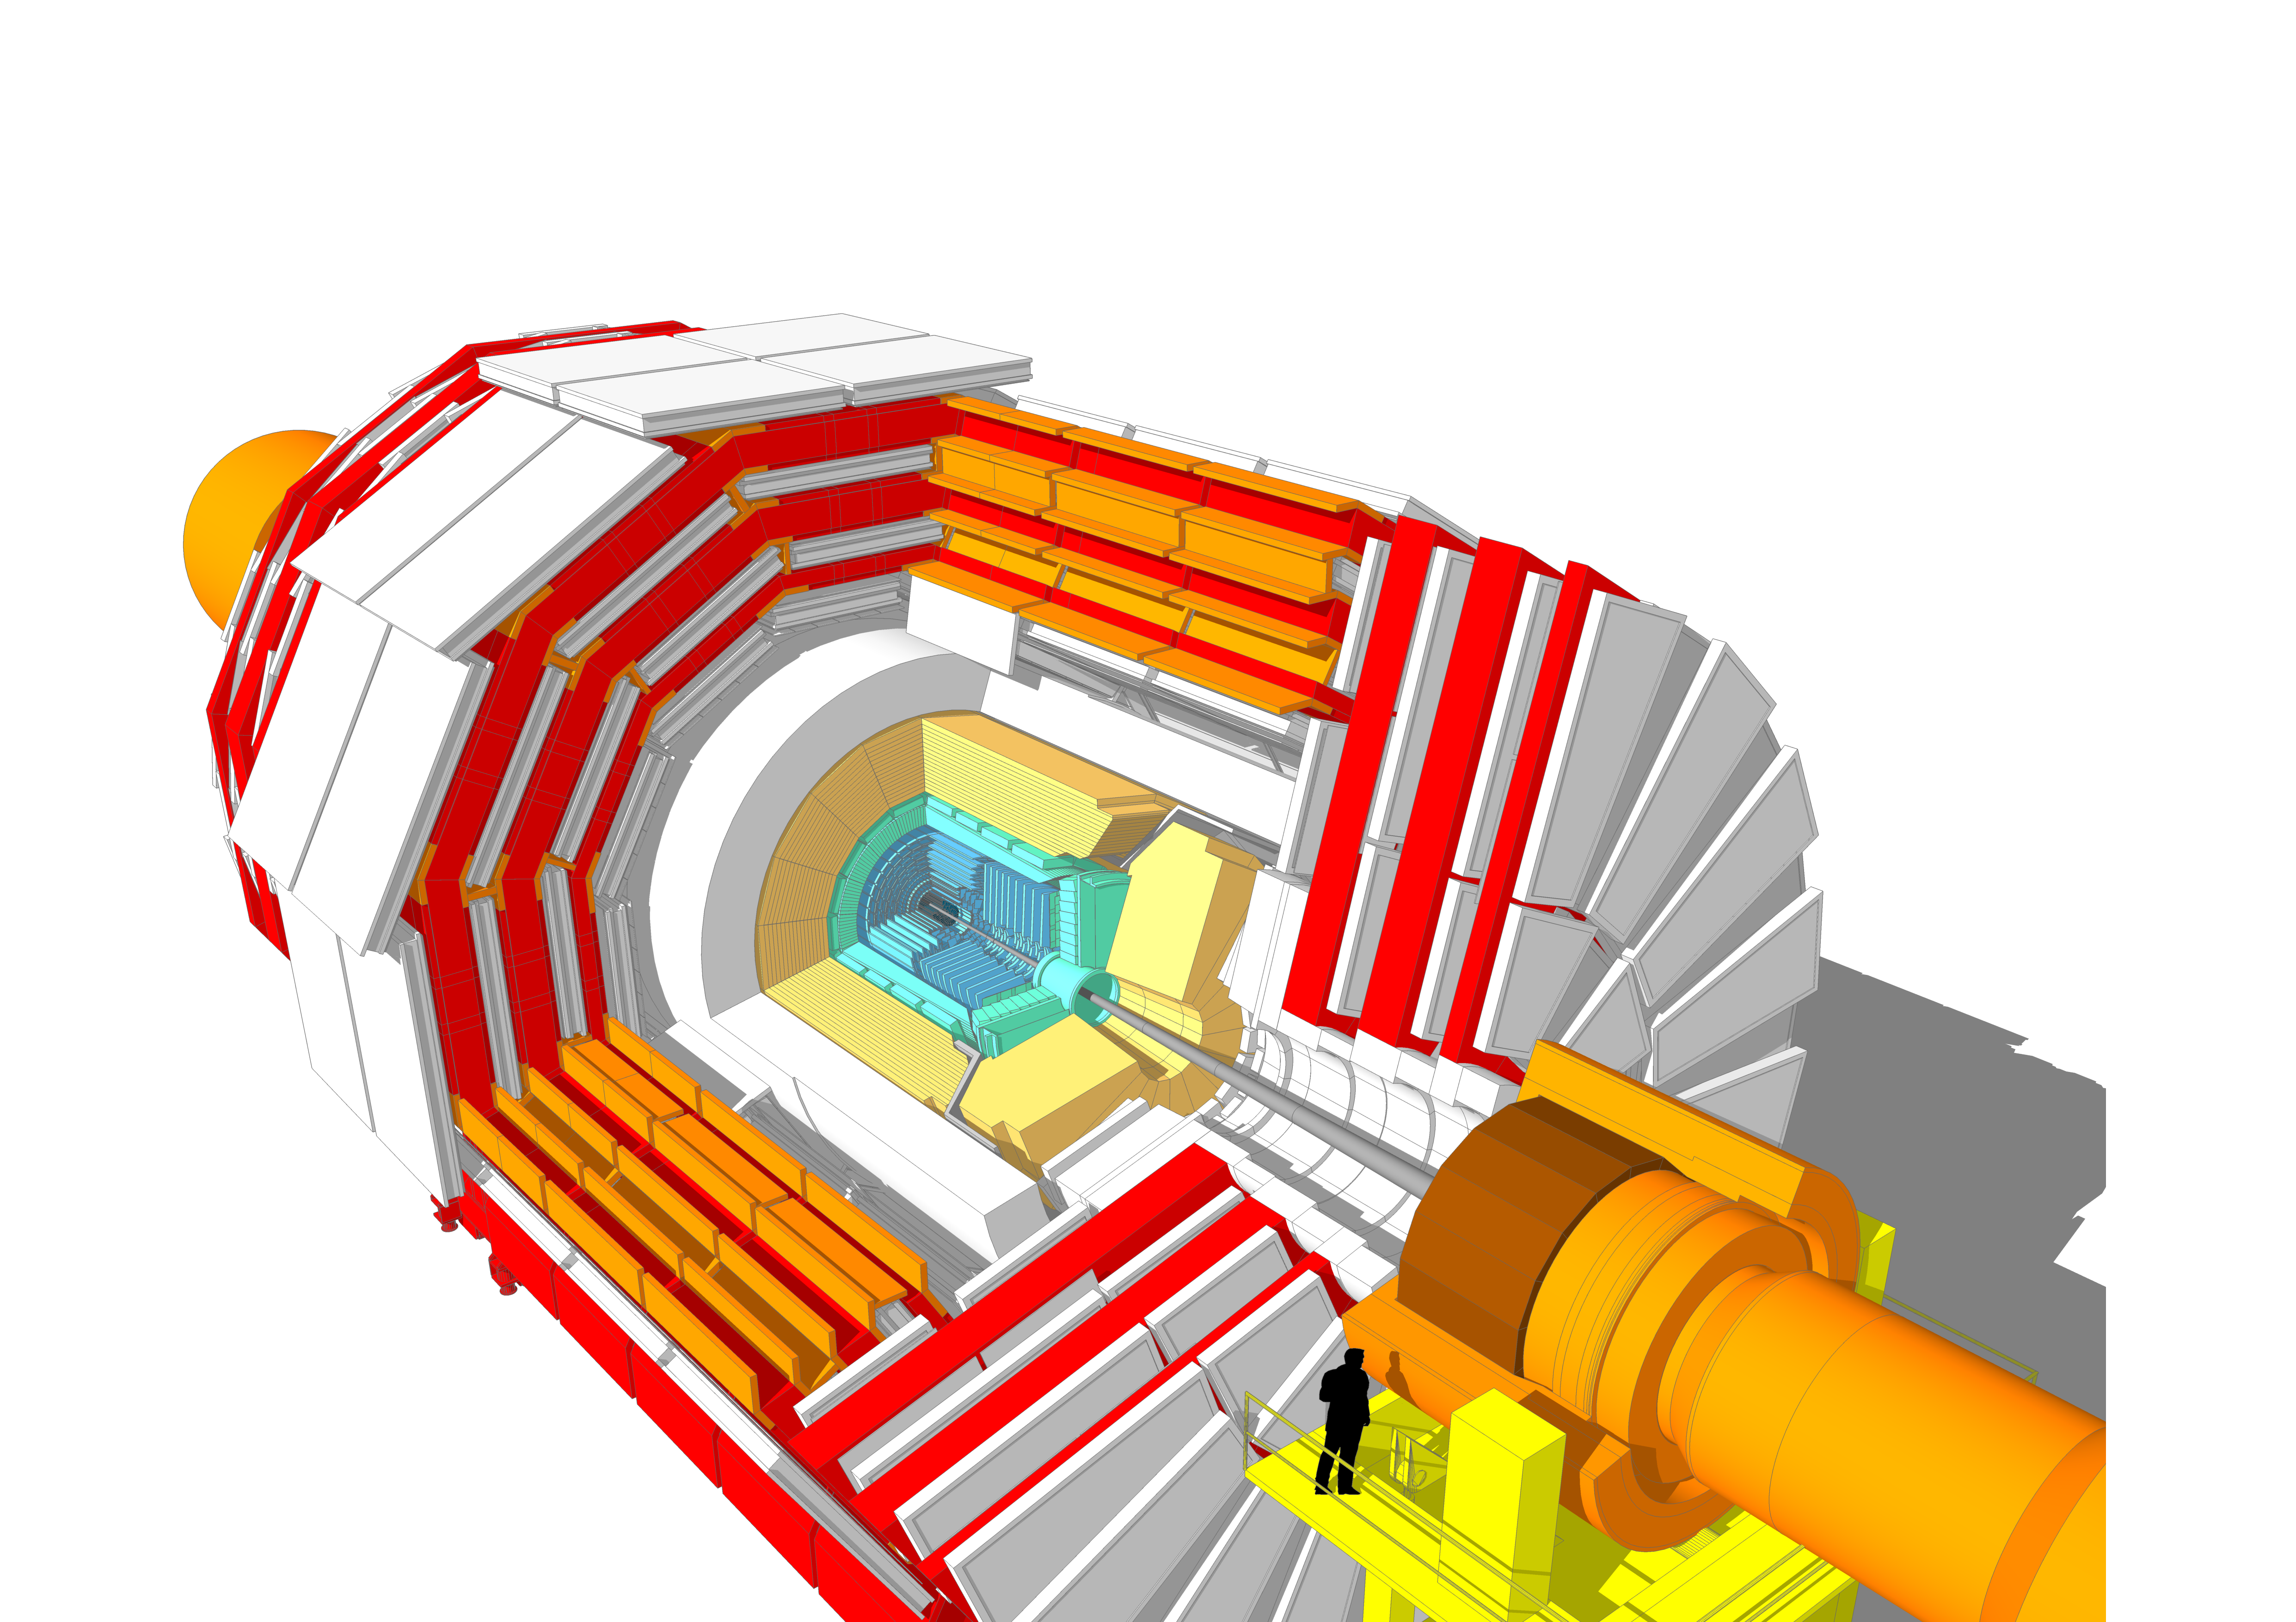
\includegraphics[width=0.95\textwidth]{pics/LHC_CMS/cms_phase1.pdf}
    \caption{A cutaway diagram of the CMS detector. 
             The design is specified to a design stage called the Phase-1 detector upgrade~\cite{arXiv:2012.14304, Mans:1481837,Tapper:1556311}.
             Plot taken from Ref.~\cite{Sakuma:2665537}.}
    \label{fig:cms_detector}
\end{figure*}

CMS adopts a spherical coordinates convention: the origin is positioned at the geometrical center of CMS expected for collisions to happen;
the $z$ axis is along the beam pipe with its positive direction pointing toward the Jura mountain;
the $\phi = 0$ direction (or the $x$ axis of the Cartesian coordinates) points horizontally toward ATLAS at the opposite side of the LHC tunnel;
this leaves the $y$ axis of the Cartesian coordinates pointing upward to the sky.
In addition, the polar angle $\theta$ is in most cases replaced by a variable called pseudorapidity $\eta$, 
defined as $\eta = -\text{ln}[\text{tan}(\frac{\theta}{2})]$.
The pseudorapidity is a good approximation of the longitudinal rapidity $y_{L}$ of particles in the CMS frame in the limit of $|\textbf{p}| \gg m$.
The CMS coordinates, along with the $\eta - \theta$ correspondence, are shown in Figure~\ref{fig:cms_longitudinal}.

\begin{figure*}[!htb]
    \centering
    \captionsetup{justification=justified}
    \includegraphics[width=0.95\textwidth]{pics/LHC_CMS/CMS_longitudinal.png}
    \caption{A longitudinal section view of the CMS detector, gridded with the CMS coordinates.
             Plot taken from Ref.~\cite{Sirunyan_2018}.}
    \label{fig:cms_longitudinal}
\end{figure*}


\subsection{Solenoid magnet}\label{sec:magnet}

The solenoid magnet of CMS is based on the same material as the LHC magnets, operating also at 1.9 K.
During its full operation, the superconducting coil carries an electric current of 18500 A and stores an energy of 2.6 GJ.
It generates a homogeneous 4 T field inside its bore of 6-\meter diameter and 12.5-\meter length,
providing the functioning environment for the detector components installed inside of it.
The superconducting coil is enclosed by its iron yoke, which is the heaviest part of the CMS detector, 
weighing about 12000~t, almost twice as much iron in the Eiffel Tower.
The iron yoke guides the magnetic field outside of the coil, and in the meantime serves as the supporting frame for all other CMS detector components.
Figure~\ref{fig:cms_field} shows the operating magnetic field of CMS.

\begin{figure*}[!htb]
    \centering
    \captionsetup{justification=justified}
    \includegraphics[width=0.95\textwidth]{pics/LHC_CMS/CMS_field.png}
    \caption{The magnetic field in CMS displayed in a longitudinal section, operating with a central field strength of 3.8 T.
             The field value $|B|$ is shown on the left and the field lines are shown on the right.
             Plot taken from Ref.~\cite{Collaboration_2010}. }
    \label{fig:cms_field}
\end{figure*}


\subsection{Silicon tracker}\label{sec:tracker}

The CMS inner tracker is designed to provide a precise and efficient measurement of the trajectories of charged particles emerging from the LHC collisions.
It is laid out in a cylindrical volume of 5.8-\meter length and 2.5-\meter diameter surrounding the beam pipe, shown in Figure~\ref{fig:cms_tracker}.
It is composed of a pixel detector with four barrel layers at radii of 2.9~\cm, 6.8~\cm, 10.9~\cm, and 16.0~\cm~\cite{phase1_tracker},
and a silicon strip detector with 4 + 6 barrel layers extending to a radius of 1.1~\meter~\cite{Collaboration_2008}.
Each system is completed by endcaps which consist of three disks in the pixel detector and 3 + 9 disks in the strip detector.
The CMS tracker has about 124 million pixels channels and about 9.3 million strip channels in total,
and provides its full tracking ability up to a pseudorapidity range of $|\eta| < $2.5.

\begin{figure*}[!htb]
    \centering
    \captionsetup{justification=justified}
    \includegraphics[width=0.95\textwidth]{pics/LHC_CMS/Phase1_Tracker.pdf}
    \caption{Sketch of one quarter of the Phase-1 CMS tracking system in r-z view.
             The pixel detectors are shown in green, 
             while single-sided and double-sided strip modules are depicted as red and blue segments, respectively.
             Plot taken from Ref.~\cite{phase1_tracker}.}
    \label{fig:cms_tracker}
\end{figure*}

In the pixel detector, the standard pixel size is 100 $\times$ 150 $\mum^{2}$ in $r\phi \times z$ plane, with a thickness of 285~\mum.
At the nominal LHC luminosity, about 1000 charged particles are produced in each bunch crossing, 
corresponding to a hit occupancy of the order $10^{-4}$ per pixel per bunch crossing.

At its operation, a charged particle usually generate signals in a few neighboring pixels, known as the charge-sharing.
The pixel system reads with analog pulse height readout, which enables an interpolation between the neighboring pixels
and achieves a spatial resolution in the range of 15-20~\mum.

The strip detector is made up of two subsystems in two regions, the inner region ($20 \cm < r < 55 \cm$) 
and the out region ($55 \cm < r < 110 \cm$), both composed of silicon micro-strip detectors. 
A typical micro-strip cell in the inner region has a thickness of 320 \mum and size of 10~\cm~$\times$~80~\mum,
leading to an occupancy of of up to 2-3\% per strip per LHC bunch crossing.
Micro-strip cells in the outer region, given the larger radii and reduced particle density, are larger in size:
500 \mum in thickness and up to about $25 \cm \times 180 \mum$ in size,
and corresponding to an occupancy of about 1\%.
The spatial resolution of the strip cells, after the interpolation of charge-sharing, 
ranges from 23-35~\mum in the inner barrel layers, and from 35-53~\mum in the outer barrel layers.  

All strip cells are placed parallel to the beam pipe in the barrel, and along the radial direction in the endcaps.
To provide a measurement of the coordinate along the strip length (z in the barrel and r in the endcaps),
some layers of the strip detector are constructed with a double-strip design, 
in which a second micro-strip detector module is mounted back-to-back to each original strip module with a stereo angle of 100 mrad. 
This measurement achieves a resolution of 230~\mum in the inner barrel and 530~\mum in the outer barrel, 
while the resolution varies in the endcap disks depending on the hit location.

The whole tracking system, consisting of the numerous silicon sensors and their readout system,
consumes about 60~kW of electric power, which in turn is dissipated as heat in the tracker volume.
A cooling system is built to maintain its operation temperature of -10~${}^{\circ}$C, 
in which the pixel layers are cooled with aluminum conducting tubes, 
and the strip layers are cooled with a continuous flow of $\text{C}_{6}\text{F}_{14}$ liquid.


\subsection{Calorimeters}\label{sec:calos}

The tracker provides high precision measurements on the charged particles but does not distinguish their particle type.
It does not acquire information on the numerous neutral particles like photons and neutral hadrons, either.
Calorimeters are placed outside of the tracker to absorb most types of particles and provide energy measurements on them.
Photons and electrons interact with matter primarily through the electromagnetic interaction, 
where photons convert into electron-positron pairs while electrons (and positrons) emit bremsstrahlung photons.
As a result, a photon or electron incident to thick material turns into a cascade of photons and electrons, called the electromagnetic shower.
Similarly, hadrons interact primarily with nuclei in matter through the strong interaction,
where multiple secondary hadrons are produced, which in case of dense material form a cascade of hadrons called the hadronic shower.
The spatial developments of the electromagnetic shower and hadronic shower are characterized by the radiation length ($X_{0}$) and the nuclear interaction length ($\lambda_{I}$), respectively.
CMS contains a specialized electromagnetic calorimeter (ECAL) and hadronic calorimeter (HCAL) to initiate and measure these two types of showers,
and in turn measure the energies of the corresponding particle types.
$X_{0}$ is in general much smaller than $\lambda_{I}$, therefore the ECAL in placed on the inside of the HCAL.

% ECAL
\begin{figure*}[!htb]
    \centering
    \captionsetup{justification=centering}
    \includegraphics[width=0.75\textwidth]{pics/LHC_CMS/ECAL.jpg}
    \caption{Schematic view of the CMS ECAL.
             Plot taken from Ref.~\cite{BROWN200729}.}
    \label{fig:cms_ecal}
\end{figure*}

The ECAL is a hermetic homogeneous calorimeter made of 75848 lead tungstate ($\text{PbWO}_{4}$) crystals,
61200 of which are mounted in the barrel part and 7324 in each of the two endcaps.
It is laid out in a cylindrical volume encircling the tracker, as shown in Figure~\ref{fig:cms_ecal}. 
The barrel part of the ECAL~(EB) covers the pseudorapidity range of $|\eta| < 1.479$, 
with a granularity of 360-fold in $\phi$ and $2 \times 85$-fold in $\eta$.
They are mounted not exactly toward the collision region but with a small angle of $3^{\circ}$ in both the $\phi$ and $\eta$ projections.
This avoids the intermodule cracks aligning with potential particle trajectories and creating blind regions.
The front faces of the crystals are at a radius of 1.29~\meter.
Each barrel crystal has a cross section of $22 \times 22 \mm^{2}$ at the front face and $26 \times 26 \mm^{2}$ at the rear face, and a length of 230~\mm ($25.8 X_{0}$). 
$\text{PbWO}_{4}$ has a density of $8.28 g/\cm^{3}$, and overall the barrel crystals weigh 67.4~t.
The endcap ECAL~(EE) covers the pseudorapidity range of $1.479 < |\eta| < 3.0$,
with the front faces of crystals 315.4~\cm away from the collision region in the longitudinal direction. 
The endcap crystals have an identical shape, with a cross section of $28.62 \times 28.62 \mm^{2}$ at the front face and $30 \times 30 \mm^{2}$ at the rear face, and a length of 220~\mm ($24.7 X_{0}$).
The crystals are grouped in mechanical units of $5 \times 5$ crystals arranged in a rectangular $x-y$ grid.
All crystals point at a focus 1300~\mm beyond the collision region, 
so that the intermodule cracks are $2^{\circ} - 8^{\circ}$ tilted from the directions to the collision region.
Each endcap is divided into 2 semicircles called $Dees$, each containing 138 standard $5 \times 5$ units and 18 partial units on the inner and outer circumferences.
The two endcaps together weigh 24.0~t.

$\text{PbWO}_{4}$ is a optically transparent material which scintillates at a wavelength of 420-430~\nm when excited by electrons and photons passing through it.
The crystals have a refractive index of $n = 2.29$ around the scintillation wavelength, and are optically isolated from each other.
Photons undergo total internal reflection in the crystal and are collected by the photodetector installed at the rear face of the crystal.  
The number of scintillation photons emitted by the crystals and the amplification of the photodetectors are both temperature dependent.
To maintain the stability of the ECAL performance, the operation temperature of the ECAL is kept precisely within $18 \pm 0.05^{\circ}C$
by constant $18^{\circ}C$ water flows which thermally couple to the crystals and electronics via aluminum grids.

The ECAL resolution is affected by several factors: 
the stochastic fluctuation in the shower containment, in photostatistics, and in the energy absorbed by preceding detector material along the particle trajectory; 
the noises in electronics and from pileup interactions;
and the constant error in the crystal non-uniformity and in detector calibration.
Overall, the resolution response and can be parametrized as:
\begin{equation}\label{eq:ecal_reso}
    ( \frac{\sigma}{E} )^{2} = ( \frac{S}{\sqrt{E}} )^{2} + ( \frac{N}{E} )^{2} + C^{2}
\end{equation}
in which $\sigma$ is the resolution, $E$ is the deposit energy,
$S$ is the stochastic term with an empirical value of 2.8\%, 
$N$ is the noise term with an empirical value of 12\%,
and $C$ is the constant term with an empirical value of 0.3\%.

In addition to the crystals, a preshower detector is placed in front of each ECAL endcap. 
It is a sampling calorimeter covering a pseudorapidity range of $1.653 < |\eta| < 2.6$, 
consisting of two layers of lead radiator + silicon strip sensor composite. 
The lead radiator initiate electromagnetic showers from incoming photons and electrons and the strip sensors measure the shower energy without absorbing them.
Each strip is 1.9~\mm wide, and the strip orientation in the two layers are orthogonal.
This provides a much better spatial resolution than the crystals and significantly improves the 
identification of photons from collinear photon pairs produced by the decay of neutral pions.


% HCAL
\begin{figure*}[!htb]
    \centering
    \captionsetup{justification=justified}
    \includegraphics[width=0.95\textwidth]{pics/LHC_CMS/HCAL.png}
    \caption{Schematic view of one quarter of the Phase-1 CMS HCAL in r-z view,
             showing the locations of the HB, HE, HO, and HF calorimeters.
             Plot taken from Ref.~\cite{Mans:1481837}.}
    \label{fig:cms_hcal}
\end{figure*}

The HCAL is designed to absorb and measure hadrons produced in $pp$ collisions.
It consists four main parts: a barrel calorimeter (HB) placed in between the outer extent of the EB (at $R = 1.77 \meter$) and the inner extent of the magnet coil (at $R = 2.95 \meter$),
two endcap calorimeters (HE) located in between the rear of the EE (at $z = \pm 3.9 \meter$) and the front of the first endcap muon station (at $z = \pm 5.6 \meter$),
an outer calorimeter (HO) installed outside of the solenoid complementing the HB,
and two forward forward calorimeters (HF) outside of the last endcap muon station at $z = \pm 11.2 \meter$ around the beam pipe.
The layout of these HCAL components are shown in Figure~\ref{fig:cms_hcal}.
The HB and HO covers the pseudorapidity range of $|\eta| < 1.3$, the HE covers $1.3 < |\eta| < 3.0$,
and the HF covers $3.0 < |\eta| < 5.2$.

The HB consists of 36 identical azimuthal wedges, each divided into 4 sectors in $\phi$ and 16 sectors in $\eta$.
The wedges ar constructed out of 16 flat absorber plates aligned parallel to the beam axis, each has a thickness of 40-75~\mm.
The front and rear plates are made of stainless steel, while the other 14 plates in between are made of brass.
The total absorber thickness ranges from 5.4 to 10.3 $\lambda_{I}$ depending on $\eta$, and the ECAL in front adds about another 1.1 $\lambda_{I}$ of material.
The hadronic energy deposits are sampled by 17 scintillator layers inserted in between the absorber plates (including the front and rear surfaces).
The scintillator material is called Kuraray SCSN81, with optical fibers embedded to guide the light.
The two outermost scintillator layers are 9~\mm thick while the other layers are 3.7~\mm.
The HE is built with a similar design with 17 interposing 79-\mm brass plates and 3.7-\mm SCSN81 scintillators, summing to a thickness of about 10 $\lambda_{I}$.
It consists 36 azimuthal wedges, each has 5 divisions between $1.3 < |\eta| < 1.6$ and 9 divisions between $1.6 < |\eta| < 3.0$.

The HO sits outside of the solenoid coil, which adds about $1.4 / sin\theta$ interaction lengths before HO.
The HO is geometrically aligned with the muon system and has 5 2.536-\meter-wide rings along $z$-axis.
Each ring has a single-layer scintillator at $r = 4.07 \meter$.
In particular, the HB has the minimal absorber depth near $\eta = 0$ therefore the central ring has 
two layers of scintillators at $r = 3.82 \meter$ and $4.07 \meter$, sandwiching an additional 19.5~\cm thick piece of iron.
HO rings are divided into 12 identical $\phi$ sectors and each sector is further divided into 6 slices.
Each slice is in turn divided into basic units called tiles along $\eta$, with 8 divisions in ring 0, 6 divisions in rings $\pm 1$, and 5 divisions in rings $\pm 2$. 

The HF is overall a cylindrical structure with an outer radius of 130.0~\cm and an inner bore radius of 12.5~\cm to accommodate the beam pipe.
Each HF calorimeter is divided into 18 equal wedges in $\phi$ and 13 units, known as towers, with roughly equal $\eta$ intervals. 
Each tower is made of a bundle of quartz fibers which run parallel to the beam line.
Quartz is chosen because of its resilience to harsh radiation environment in the forward region:
on average 760~\GeV of energy per $pp$ collision is deposited into the HF, while 100~\GeV is distributed in the rest of the detector.
Signals are detected not as hadronic showers but as the Cherenkov radiation generated by charged particles in the quartz medium, 
therefore the HF is insensitive to neutral hadrons.
The whole cylindrical structure is housed in a hermetic radiation shielding consisting of composite layers of steel, concrete and polyethylene. 

Overall, HCAL has a granularity of $\Delta\eta \times \Delta\phi = 0.087 \times 0.087$ for $|\eta| < 1.6$ (HB and HE), 
$0.17 \times 0.17$ for $1.6 < |\eta| < 3.0$ (HE), and $0.175 \times 0.175$ for $3.0 < |\eta| < 5.0$ (HF).


\subsection{Muon detectors}\label{sec:muon_chambers}

Muon detection at CMS, as implied by its name, is of central goal of its design.
CMS uses three types of gaseous particle detectors for muon detection in its original design:
drift tubs (DT), cathode strip chambers (CSC), and resistive plate chambers (RPC).
Additional gas electron multipliers (GEM) are installed in 2019 as a part of the phase-2 upgrade plan of CMS. 
The locations of different muon detectors are shown in Figure~\ref{fig:cms_muons}.

\begin{figure*}[!htb]
    \centering
    \captionsetup{justification=justified}
    \includegraphics[width=0.95\textwidth]{pics/LHC_CMS/muon_chambers.png}
    \caption{A longitudinal section view of the current CMS detector specifying the locations of muon chambers.
             This plot is different from Figure~\ref{fig:cms_longitudinal} only by the GEM detector installed in 2019.
             Plot taken from Ref.~\cite{Colaleo:2021453}.}
    \label{fig:cms_muons}
\end{figure*}



The muon system consists of a barrel section and two endcaps, each of them containing four layers of composite detectors, 
called stations, interleaved with the return yoke of the solenoid magnet.
The barrel of the muon system covers $|\eta| < 1.2$ with 5 wheels along the $z$ direction.
Each wheel consists 4 stations along the $r$ direction and each station is made of 12 sectors.
Each sector is a planar structure parallel to $z$ and perpendicular to $r$, 
and the 12 of them together encircle the barrel.
In each sector, there are one DT layer and one or two RPC layers: the DT in the first and second stations is sandwiched by two layers of RPC,
while the DT in the third and fourth stations is only accompanied with a RPC layer on the inner side of it.
The muon endcaps cover $0.9 < |\eta| < 2.4$, forming an overlap with the barrel to make sure there is no acceptance gap.
Each endcap is a disk with 4 stations of muon chambers.
Each station is divided into 2 or 3 rings (3 for the first station and 2 for the others), and each ring consists six $60^\circ$ sectors.
In each sector, there are six $10^\circ$ CSC chambers except for the inner ring of stations 2-4 which have three $20^\circ$ degree chambers.
The CSC chambers in the inner ring of the first station (ME1/1) are accompanied with GEM chambers whose boundaries are aligned with the CSC chambers.
The CSC chambers in the outer rings of station 1 and in the outer ring of stations 2-4 are accompanied with RPC chambers aligned with them.

\begin{figure*}[!htb]
    \centering
    \captionsetup{justification=justified}
    \includegraphics[width=0.45\textwidth]{pics/LHC_CMS/DT.png}
    \includegraphics[width=0.45\textwidth]{pics/LHC_CMS/DT_superlayer.png}
    \caption{Left: sketch of a cell of the drift tube detector showing drift lines and isochrones.
             Right: schematic view of DT superlayers.
             Plot taken from Ref.~\cite{collaboration_2013}.}
    \label{fig:cms_dt}
\end{figure*}

The DT chambers are arrays of rectangular drift cell, whose design is illustrated in the left plot of Figure~\ref{fig:cms_dt}.
Each cell has a transverse size of $42 \times 13 \mm^{2}$ with a 50-\mum-diameter 
gold-plated stainless steel wire positioned in the center through its full length.
A DT chamber is made of 3 (or 2 for the fourth station) superlayers, each made of 4 stacked layers of drift cells, staggered by half a cell.
The superlayers are aligned alternately along the $z$ and $\phi$ directions, shown in the right plot of Figure~\ref{fig:cms_dt}.
The cell length is 2.5~\meter for those aligned along $z$, and ranges from 1.9~\meter to 4.1~\meter for those aligned along $\phi$.
DT tubes are filled with a gas mixture of 85\% Ar and 15\% $\text{CO}_{2}$.
Electric voltages are applied to different parts in the tube to generate a certain potential gradient:
the steel wires are at $+3600$~V as the anodes, the aluminum walls on the 13-\mm sides are at $-1200$~V as the cathodes,
and the aluminum walls on the 42-\mm sides are at $+1800$~V to help guide the gradient from anodes to cathodes.

When a muon passes through DT cells, it ionize the $\text{Ar-CO}_{2}$ mixture. 
The resulting free electrons are attracted to the anodes and accelerated in the field, ionizing more gas molecules along their path.
This avalanche makes a gain about $10^5$ and leads to a detectable current as the signal.
The electron avalanche drifts at a roughly constant velocity about 50 $\mum/\ns$, 
meaning that it takes at maximum close to 400 \ns for the electric signal to develop 
(for incident muons at the farthest corners 21 \mm away from the anode wire).
This drift time is measured from the signal timing differences between the 4 staggered layers in a superlayer~\cite{ARCE2004441}.
The determination of this drift time is particularly important as the $pp$ bunch crossings are only 25 \ns apart from each other.
Overall, the DT can achieve a time resolution of about 2 \ns, which, given the constant drift velocity, 
can be translated into a spatial resolution of order 100 \mum.
However, a caveat is accompanied with this great time and spatial resolution: 
in a very unlikely case where two or more muons pass through the same drift cell in consecutive bunch crossings,
the cell may not recover from the earlier avalanche and become inefficient to the later ones.
This is mitigated by the fast-responding RPC detectors which are described later in this section.

\begin{figure*}[!htb]
    \centering
    \captionsetup{justification=justified}
    \includegraphics[width=0.90\textwidth]{pics/LHC_CMS/CSC.png}
    \caption{Left: layout of a CSC chamber showing arrangement of anode wires and cathode strips.
             Right: an illustration of the principle of CSC operation.
             Plots taken from Ref.~\cite{collaboration_2013}.}
    \label{fig:cms_csc}
\end{figure*}

The CSCs, shown as the left plot of Figure~\ref{fig:cms_csc}, are multiwire chambers comprised of 6 anode wire planes interleaved among 7 cathode strip panels.
The wires are equally spaced of about 3~\mm and run along the $\phi$ direction.  
Each cathode strip panel contains 80 strips running along the $r$ direction, each covering a constant $\phi$ interval and corresponding to a width between 3~\mm to 16~\mm. 
The gap between adjacent cathode panels (with wires in between) is about 1 \cm.  
The overall dimension of CSCs vary for different stations and rings, the largest of which is about $3.4 \times 1.5 \meter^{2}$.

A gas mixture of 40\%Ar+50\%CO$_{2}$+10\%CF$_{4}$ is filled in the CSC chambers and 
a 3.6~kV voltage difference is applied between the anodes and cathodes.
The principle for CSC operation is the same as that described for the DT.
The drift time in CSC is within a few bunch crossings as it has a shorter drift length than the DT.
After offline calibrations, the CSC can achieve a time resolution of about 3~\ns.
In particular, when electrons move toward the anode wires, charges are induced in the nearby cathode strips, as illustrated in the right plot of Figure~\ref{fig:cms_csc}.
By interpolating the distribution of these charges, a spatial resolution of the incident particle can be achieved better than the strip pitch,
as good as about 2~\mm at the trigger level and around 100~\mum in off-line reconstruction.  

\begin{figure*}[!htb]
    \centering
    \captionsetup{justification=centering}
    \includegraphics[width=0.90\textwidth]{pics/LHC_CMS/RPC.png}
    \caption{Schematic view of a double gap RPC.
             Plot taken from Ref.~\cite{collaboration_2013}.}
    \label{fig:cms_rpc}
\end{figure*}

The RPC chambers are used in both the barrel and endcaps, with their dimensions aligned with the corresponding DT or CSC chambers.
A basic double-gap RPC module is shown in Figure~\ref{fig:cms_rpc}. 
Each gas gap consists of resistive plates made of graphite-coated 2-\mm bakelite plates, 
which are separated by 2-\mm spacers and a composite gas mixture.
A layer of anode strips is inserted between the double gas gaps as the readout.
The nominal voltage applied to the outer resistive plates is 9.6~kV.

The RPC features a respond rate much shorter than 25~\ns,
which is crucial in providing bunch crossing assignment and keeping high efficiency of the overall muon system.
It spatial resolution, on the contrary, is worse than the DT and CSC, ranging between 0.8~\cm to 1.4~\cm.

\begin{figure*}[!htb]
    \centering
    \captionsetup{justification=justified}
    \includegraphics[width=0.90\textwidth]{pics/LHC_CMS/GEM.png}
    \caption{Left: schematic view showing the GEM structure and its working principle.
             Right: exploded view of the mechanical design of GEM.
             Plot taken from Ref.~\cite{Colaleo:2021453}.}
    \label{fig:cms_gem}
\end{figure*}

The GEM detectors are a new component installed in the muon endcaps in front of the CSC chambers in 2019.
At the moment only one GEM station has been installed for each endcap, as shown in Figure~\ref{fig:cms_muons}.
The basic unit of GEM is a "Triple-GEM detector", shown in Figure~\ref{fig:cms_gem}.
A triple-GEM chamber features a stack of three GEM foils placed with gaps of a few millimeter immersed in a gas mixture.
Each GEM foil is a thin metal-clad polymer foil with arrays of holes on it distributed in a hexagonal patter. 
GEM foils are encased by a drift board and a readout board which are connected to a nominal voltage difference of 3200~V.
The total distance between the drift board and the readout board is about 7~\mm.
The holes in GEM foils guides the electric field through them, providing a high avalanche amplification factor while preventing electrical breakdown problems.

The readout board is fine grained with a 300~$\mu$rad (or 0.8~\mm) precision along the $\phi$ direction.
As the GEM chamber has a short drift distance and a fast drift speed, it is fast-responding with a time resolution better than 10~\ns, 
In practice, two triple-GEM chambers are always stacked to form a superchamber, providing independent measurements.
Combination of the two measurements improves the time and spatial resolution and also recover inefficiency which are about 3\% for a single chamber.

\subsection{Trigger system}\label{sec:trigger}

LHC is an extremely busy machine colliding protons bunches with a nominal bunch spacing of 25~\ns and a nominal instantaneous luminosity of $1.0 \times 10^{34}~\cm^{-2}\text{s}^{-1}$. 
With tens of millions of readout channels in the CMS detector, it is impossible to record all collision data, which correspond to a data flow of about 50~TB/s. 
Meanwhile, most $pp$ collisions are soft scatters and do not contain physics processes of primary interests.
To reduce the intense requirement on offline storage and processing, and to filter out uninteresting collisions,
a trigger system is implemented in CMS selecting and recording only 0.0025\% of the collision events.

The CMS trigger system has two levels. 
The first level is called the Level-1 Trigger (L1T) which is built from custom electronics specialized in fast parallel processing.
It makes decisions based on signals from calorimeters and muon chambers and reduces the event rate from the collision rate of 40~MHz to below 100~kHz.
The second level is the High Level Trigger (HLT) is a software system operating on a commercial processor farm.
It utilizes the readouts from all detectors and reduces the event rate to less than 1~kHz. 

The L1T receives coarsely segmented data, known as Trigger Primitives (TP), from the calorimeters and the muon system, 
while holding the full-precision data in pipelined memory buffers corresponding to a latency of 4~\mus.
The L1T must analyze every bunch crossing and decide whether to keep the data before they are pushed out of the buffer and lost forever.
As electronic signals only travel (at the speed of light) 1200~\meter in 4~\mus, the L1T needs to be physically near the detector for swift communication.
Part of L1T electronics is installed on the CMS detector, and the rest is located in the underground control room about 90~\meter from the experimental cavern.
The full-precision data of L1T accepted events are transmitted to the above-ground computing center at a rate of about 100~GB/s and are further analyzed by the HLT. 
The HLT processes these events among more than 20000 CPU cores with the per-event processing time relaxed to O(100~\ms).
The HLT runs a full reconstruction algorithm similar to the offline reconstruction described in Section~\ref{sec:obj_reco}
and selects events based on their physics signatures. 
Events passing the HLT selection, corresponding to a data flow of a few GB/s, 
are distributed in the CERN computing grid for storage and further processing,
composing the collision dataset recorded by the CMS experiment. 

\begin{figure*}[!htb]
    \centering
    \captionsetup{justification=justified}
    \includegraphics[width=0.90\textwidth]{pics/LHC_CMS/L1T.png}
    \caption{Diagram of the CMS Level-1 trigger structure during Run 2.
             Plot taken from Ref.~\cite{l1t_perform}.}
    \label{fig:cms_l1t}
\end{figure*}

The structure of the L1T is shown in Figure~\ref{fig:cms_l1t}, 
it consists a muon trigger and a calorimeter trigger.
The muon trigger includes three muon track finders (MTF) covering the barrel (BMTF), overlap (OMTF), and endcap (EMTF) regions,
and a global muon trigger for final muon selection. 
Trigger Primitives (TP) are generated for each detector sector containing information like $\eta$, $\phi$ positions, timing (bunch crossing), and hit patterns.
The CSC TPs are track segments called local charged tracks (LCT) and are organized by the muon port cards (MPC).
The DT TPs are also track segments. 
They are combined with near by RPC hits to form superprimitives in processors called TwinMux~\cite{CMS-DP-2016-074}.
As RPC chambers have less internal layers, the RPC TPs are hits containing only position and timing information.
RPC hits in the barrel region are processed by the TwinMux, while hits in the endcaps are clustered and formatted by the concentration preprocessing and fan-out (CPPF) boards.
The BMTF takes inputs from TwinMux, the EMTF takes inputs from both MPC and CPPF, 
while the OMTF receives inputs from all these components within its coverage.
The MTFs combine TPs from different muon stations, build muon track candidates, 
evaluate their momentum, and assign a ranking based on their track qualities.
Each MTF can send up to 36 muon candidates to the global muon trigger, 
which resolves duplicates from different sources, sorts the overall ranking, 
and sends up to 8 highest ranked muons to the global trigger for final L1T decisions.

The calorimeter trigger consists two layers. 
The Layer-1 receives TPs from ECAL and HCAL and calibrates their energy deposits. 
The Layer-2 combines the calibrated TPs and reconstructs trigger objects such as electrons, photons, tau leptons, jets, and energy sums.
(Electrons and photons are indistinguishable at L1T level and are together referred to as $E/\gamma$ candidates.)
The Layer-2 is a time multiplexed trigger~\cite{Frazier_2012} in which different bunch crossings are analyzed in parallel by multiple identical boards. 
In this way each board has a more relaxed processing time and can access the full acceptance and granularity of the ECAL and HCAL.
A demultiplexer (DeMux) board summarizes, reorders, and formats the output from multiplexers and transmits the results to the global trigger.

All the mentioned L1T components are built on Xilinx Virtex-7 Field Programmable Gate Array (FPGA) boards.
This design greatly boosts the reusability and flexibility of the trigger system, and reduces the workload for development and maintenance.
The largely programmable boards also enable the application of complex multivariate algorithms at trigger level in the form of look-up tables.

The global trigger examines all muon and calorimeter objects and makes decisions based a list of trigger requirements known as the trigger menu.
The trigger menu consists of about 400 trigger seeds combined with "or" logic.
Each trigger seed is a set of requirements on the \pt, $\eta$, isolation, and other quantities of certain trigger object(s).
For example, a single muon trigger may ask for a muon with $\pt > 22$~\GeV and to be isolated from other trigger objects, 
and a single muon + double jets trigger may ask for one muon and two jets in the events that are close together.
A detailed list of trigger seeds can be found in Ref.~\cite{l1t_perform}.
The selection requirements in trigger seeds are adjusted so that the total trigger rate is contained at a reasonable level.
For some cases where there is a need to make loose selections while keeping the trigger rate low, a "prescale" method is applied.
A trigger with a prescale of $N$ means that in every $N$ events passing this trigger, only one of them is accepted and recorded.
In general, the unprescaled triggers are used to collect data for physics analyses, 
while the prescaled triggers are used for calibrations and trigger performance studies.
One extreme example of the prescaled triggers is the zero-bias trigger, 
which does not require any particular objects from the proton collisions.
It fires at a very low rate and makes the baseline dataset for various trigger studies.

The HLT menu is similar to the L1T menu but is based on much better reconstructed physics objects.
In particular, the trigger paths taken by the analysis of \hmm decay are the single isolated muon triggers 
with a \pt threshold of 24/27/24~\GeV for 2016/2017/2018 datasets.  
These single muon triggers in general have an efficiency greater than 90\% for muons above the trigger threshold. 
With two muons from the Higgs decay, the overall trigger efficiency for signal events is close to 100\% with regard to the offline analysis selection detailed in Section~\ref{sec:obj_sel}.

%\section{Level-1 Trigger}

\chapter{Overview of the search of \texorpdfstring{\hmm}{H to muons} decay at CMS}\label{chp:hmm_overview}
% Need to use \textorpdfstring{} so it also shows in pdf bookmarks 

In 2012, a new boson at 125 \GeV was discovered by ATLAS and CMS at the LHC~\cite{Aad:2012tfa, Chatrchyan:2012xdj, Chatrchyan:2013lba}. 
Various measurements have been performed to probe the properties of this boson ever since, 
and the boson was later acknowledged as the Higgs boson predicted by the SM.
Up to now, the couplings between the Higgs boson and the electroweak (EW) gauge bosons have been observed to be consistent with the SM prediction, 
while the Yukawa couplings between the Higgs boson and the fermions have only been established for the third generation fermions. 
The first and second generation fermions are less massive than their third generation counterparts and thus weaker coupling to the Higgs boson, 
as the coupling strength is proportional to the mass of the fermion.
This leads to significantly smaller branching fractions of the decay modes of the Higgs boson to the first or second generation fermions, 
and poses a substantial challenge to the searches for such decays.  
The \hmm decay in particular, has a branching ratio of ${\brhmm = 2.18 \times 10^{-4}}$, 
which corresponds to an expectation of about 1000 event instances in all the data collected by CMS from 2016 to 2018 (called the LHC Run 2 data-taking period).
In contrast, these 1000 so-called signal events are engulfed by millions of events produced through other processes (background events) that mimic their experimental signature.
The search for the \hmm decay, in a nutshell, is a struggle to make the signal events stand out from the vast backgrounds with statistical significance.

The search for the \hmm decay has been conducted using proton-proton ($pp$) collision data collected at center-of-mass energies of 7, 8, and 13 \TeV
by the CMS Collaboration~\cite{2015184, PhysRevLett.122.021801} and the ATLAS Collaboration~\cite{201468, PhysRevLett.119.051802, Aad:2020xfq}.
The latest result~\cite{PhysRevLett.122.021801} from CMS prior to this work reported an observed (expected in absence of \hmm decay) upper limit of 2.9 (2.2) times the 
SM prediction of the Higgs boson production and the \brhmm, at the 95\% confidence level (CL).

Despite the challenging nature of the \hmm analysis, many efforts can be made to improve the separation of signal and background processes, 
allowing for a sizable refinement of the result.
First of all, the Higgs boson has a narrow natural width, and the muons are well identified objects in the CMS detector.
This means that the two muons from the Higgs decay always compose an invariant mass near the nominal Higgs mass, 125 \GeV.
While for the background processes, the muons are created either by the decay of a \PZ boson, 
or by decays of multiple particles, for example a \Pqt and \Paqt quark pair, each resulting in a single muon.
The \PZ boson has a mean mass at 91.2 \GeV and a natural width of 2.5 \GeV, making a slowly falling tail in the mass spectrum around 125 \GeV.
For the muons that come from two different sources, their invariant mass follows a flat random distribution near the mass range of interest.
Therefore, the signal can be strongly distinguished against the background in the dimuon invariant mass spectrum, 
as a sharp peak against a smooth falling shape. Figure~\ref{fig:dimuon_mass_shapes} shows the conceptual shape of these mass spectra. 

\begin{figure}[!htb]
    \centering
    \captionsetup{justification=justified}
    \includegraphics[width=0.6\textwidth]{pics/hmm_mass_sketch.png}
    \caption{A conceptual plot for the dimuon mass shapes for the signal and the background. 
             The blue line shows the expected background shape, while the red line shows the expected signal shape on top of it.}
    \label{fig:dimuon_mass_shapes}
\end{figure}

Furthermore, the Higgs boson is produced via several distinct production modes, each with some unique kinematic characteristics. 
By applying selection criteria targeting a certain signal production mode, it is possible to select a specific part of the kinematic phase space that is enriched with that signal, 
and reject many background processes that do not share the same kinematic features. 
There are four main production modes considered in this analysis, ordered by their production cross sections: gluon fusion (\ggH), vector boson fusion (\qqH or qqH), 
associated production with a weak vector boson (\VH), and associated production with a pair of top quarks (\ttH). 
The Feynman diagrams for these main production modes are shown in Figure~\ref{fig:main_higgs_modes}.
Some other minor production modes are also considered as signal contributions, including associated production with a pair of bottom quarks (\bbH),
associated production with a \PZ boson through gluon fusion (\ggZH), associated production with a top quark and a \PW boson (\tHW), 
and associated production with a top quark and a light quark (\tHq). 
The Feynman diagrams for these minor production modes are shown in Figure~\ref{fig:minor_higgs_modes}.
Table~\ref{tab:signal_xsec} summarizes the cross sections for all these production modes, 
along with the expected number of events in the Run 2 dataset (137 \invfb).

\begin{figure}[!htb]
    \centering 
    \captionsetup{justification=centering}
    \begin{subfigure}[b]{0.45\textwidth} % b for bottom alignment so caption is at the same height
        \centering
        \feynmandiagram[horizontal=g1 to t1, horizontal=t2 to h] {
            g1 [particle = \Pg] -- [gluon] t1,
            t1 -- [fermion, edge label = \Pqt] t2 -- [fermion, edge label = \Pqt] t3 -- [fermion, edge label = \Pqt] t1,
            g2 [particle = \Pg] -- [gluon] t3,
            t2 -- [scalar] h [particle = \PH],
            g1 -- [draw=none] g2,
        };

        \caption*{\ggH}
    \end{subfigure} 
    %to put these two diagrams side by side. no empty line in between these two blocks, otherwise it indicates an empty line in the pdf
    \begin{subfigure}[b]{0.45\textwidth}
        \centering
        \feynmandiagram[horizontal=b to h]{
            q1 [particle = $\Pq_{1}$] -- [fermion] a -- [fermion] aq1 [particle = $\Pq^\prime_{1}$],
            a -- [boson, edge label = \PV] b -- [boson, edge label = \PV] c,
            b -- [scalar] h [particle = \PH],
            aq2 [particle = $\Pq_{2}$] -- [fermion] c -- [fermion] q2 [particle = $\Pq^\prime_{2}$],

            q1 -- [draw = none] n -- [draw = none] aq2,
            a -- [draw = none] c,
            aq1 -- [draw = none] h -- [draw = none] q2,

        };
        \caption*{\qqH}
    \end{subfigure}

    \begin{subfigure}[b]{0.45\textwidth}
        \centering
        \feynmandiagram[horizontal=a to b] {
            q [particle = \Pq] -- [fermion] a -- [anti fermion] aq [particle = $\Pq^\prime$],
            a -- [boson, edge label = \PV] b,
            v [particle = \PV] -- [boson] b -- [scalar] h [particle = \PH],
        };
        \caption*{\VH}
    \end{subfigure}
    \begin{subfigure}[b]{0.45\textwidth}
        \centering
        \feynmandiagram[horizontal=b to h]{
            g1 [particle = \Pg] -- [gluon] a -- [fermion] t1 [particle = \Pqt],
            a -- [anti fermion, edge label = \Paqt] b -- [anti fermion, edge label = \Pqt] c,
            b -- [scalar] h [particle = \PH],
            g2 [particle = \Pg] -- [gluon] c -- [anti fermion] t2 [particle = \Paqt],

            g1 -- [draw = none] n -- [draw = none] g2,
            a -- [draw = none] c,
            t1 -- [draw = none] h -- [draw = none] t2,
        };
        \caption*{\ttH}
    \end{subfigure}
    \caption{Main production modes of the Higgs boson.}
    \label{fig:main_higgs_modes}
\end{figure}



\begin{figure*}[!htb]
    \centering
    \captionsetup{justification=centering}
    \begin{subfigure}[b]{0.45\textwidth}
        \centering
        \feynmandiagram[horizontal=b to h]{
            g1 [particle = \Pg] -- [gluon] a -- [fermion] b1 [particle = \Pqb],
            a -- [anti fermion, edge label = \Paqb] b -- [anti fermion, edge label = \Pqb] c,
            b -- [scalar] h [particle = \PH],
            g2 [particle = \Pg] -- [gluon] c -- [anti fermion] b2 [particle = \Paqb],

            g1 -- [draw = none] n -- [draw = none] g2,
            a -- [draw = none] c,
            b1 -- [draw = none] h -- [draw = none] b2,
        };
        \caption*{\bbH}
    \end{subfigure}
    \begin{subfigure}[b]{0.45\textwidth}
        \centering
        \feynmandiagram[horizontal=a to b] {
            g [particle = \Pg] -- [gluon] a -- [anti fermion] qb [particle = \Pqb],
            a -- [fermion, edge label = \Pqb] b,
            w [particle = $\PW^{-}$] -- [boson] b -- [fermion, edge label = \Pqt] th -- [fermion] t [particle = \Pqt],
            th -- [scalar] h [particle = \PH],
            t -- [draw = none] h -- [draw = none] w, 
        };
        \caption*{\tHW}
    \end{subfigure}

    \begin{subfigure}[b]{0.45\textwidth}
        \centering
        \feynmandiagram[vertical=a to b] {
            q [particle = \Pq] -- [fermion] a -- [fermion] aq [particle = \Pq'],
            a -- [boson, edge label = \PW] b,
            qb [particle = \Pqb] -- [fermion] b -- [fermion, edge label = \Pqt] c,
            c -- [scalar] h [particle = \PH],
            c -- [fermion] t [particle = \Pqt],
            q -- [draw = none] n -- [draw = none] qb,
            aq -- [draw = none] h -- [draw = none] c,
            aq -- [draw = none] h -- [draw = none] t,
        };
        \caption*{\tHq}
    \end{subfigure}
    \begin{subfigure}[b]{0.45\textwidth}
        \centering
        \feynmandiagram[horizontal=b to h]{
            q1 [particle = \Pq] -- [fermion] a -- [fermion] q2 [particle = $\Pq^\prime$],
            a -- [boson, edge label = \PW] b -- [boson, edge label = \PW] c,
            b -- [scalar] h [particle = \PH],
            qb [particle = \Pqb] -- [fermion] c -- [fermion] qt [particle = \Pqt],

            q1 -- [draw = none] n -- [draw = none] qb,
            a -- [draw = none] c,
            q2 -- [draw = none] h -- [draw = none] qt,
        };
        \caption*{\tHq}
    \end{subfigure}

    \begin{subfigure}[b]{0.45\textwidth}
        \centering
        \feynmandiagram[horizontal=g1 to q1, horizontal=q2 to z] {
            g1 [particle = \Pg] -- [gluon] q1,
            q1 -- [fermion, edge label' = \Pq] q2 -- [fermion, edge label' = \Pq] q3 -- [fermion, edge label' = \Pq] q1,
            g2 [particle = \Pg] -- [gluon] q3,
            q2 -- [boson, edge label = \PZ] z ,
            z -- [boson] z2 [particle = \PZ],
            z -- [scalar] h [particle = \PH],
            g1 -- [draw=none] g2,
        };
        \caption*{\ggZH}
    \end{subfigure} 
    \begin{subfigure}[b]{0.45\textwidth}
        \centering
        \feynmandiagram[horizontal=t1 to t2] {
            g1 [particle = \Pg] -- [gluon] t1 -- [fermion, edge label = \Pqt] t2 -- [boson] z [particle = \PZ],
            g2 [particle = \Pg] -- [gluon] t4 -- [anti fermion, edge label = \Pqt] t3 -- [scalar] h [particle = \PH],
            t1 -- [anti fermion, edge label = \Pqt] t4,
            t2 -- [fermion, edge label = \Pqt] t3,
            g1 -- [draw = none] g2,
            z -- [draw = none] h,
        };
        \caption*{\ggZH}
    \end{subfigure} 
    \caption{Examples of minor Higgs production modes.}
    \label{fig:minor_higgs_modes}
\end{figure*}

\begin{table}[!htb]
    \centering
    \captionsetup{justification=justified}
    \topcaption{Production modes of the Higgs boson in $pp$ collisions at the LHC, their cross sections for $\mh = 125 \GeV$, 
                and the corresponding expected number of events in the dataset for this analysis 
                (the cross sections multiplying \brhmm and the integrated luminosity ($137 \invfb$). 
                The leptons ($\ell$) in the table refer to electrons or muons.}
    \begin{tabular}{lccc}
        \hline
        signal mode         & decay mode                & Cross section (\pb)   & Expected number of events \\
        \hline
        \ggH                & inclusive                 & 48.58                 & 1450 \\
        \qqH                & inclusive                 & 3.782                 & 113 \\
        \WH                 & inclusive                 & 1.373                 & 41.0 \\
                            & $\PW\to\ell\nu$           & 0.293                 & 8.75 \\
%                            & $\PW\to$ hadrons          & 0.926                 & 27.6 \\
        ${\Pq\Pq\to\PZ\PH}$ & inclusive                 & 0.761                 & 22.7 \\
                            & $\PZ\to\ell\ell$          & 0.051                 & 1.53 \\
%                            & $\PZ\to\nu\nu$            & -                     & - \\
%                            & $\PZ\to$ hadrons          & -                     & - \\
        \ggZH               & inclusive                 & 0.123                 & 3.67 \\
                            & $\PZ\to\ell\ell$          & 0.008                 & 0.25 \\
%                            & $\PZ\to\nu\nu$            & -                     & - \\
%                            & $\PZ\to$ hadrons          & -                     & - \\
        \ttH                & inclusive                 & 0.507                 & 15.1 \\
                            & $\geq 1~\Pqt\to$ leptons  & 0.193                 & 5.76 \\
                            & Both $\Pqt\to$ hadrons    & 0.230                 & 6.86 \\
        \hline
        sum of above        & inclusive                 & 55.13                 & 1646 \\
        \hline
        \bbH                & inclusive                 & 0.488                 & 14.6 \\
        \tHq                & inclusive                 & 0.074                 & 2.21 \\
        \tHW                & inclusive                 & 0.015                 & 0.45 \\
        \hline
        sum of all          & inclusive                 & 55.70                 & 1663 \\
        \hline
    \end{tabular}
    \label{tab:signal_xsec}
\end{table}

Four event categories are defined in this analysis targeting each of the four main Higgs production modes,
all of them requiring two oppositely charged (OS) muons that form a candidate for the Higgs boson decay.
The additional requirements for each category are:
the \ttH category requires the presence of additional b-jets (from the decay of the top quarks) in the event,
the \VH category targets events with additional leptons (\Pe or \mu, from the decay of the vector boson), 
the \qqH category selects events with two energetic and forward jets,
while the \ggH category does not specify additional objects, and collects all events that are not selected by the other three categories.
No dedicated category is made for the minor signal modes, either because they have very similar features to one of the main modes, 
or because their cross sections are much smaller than the main modes and do not make a difference.

With such selections, naturally, each of the selected phase spaces presents a distinct event topology and contains a distinct background composition. 
Therefore, the analysis is performed independently in each of the event categories, following different optimized strategies. 
The detailed description of the analysis strategies in each event category is given in Section~\ref{sec:hmm_cat_and_strategy}.

\bigskip
\section{Data and simulation samples}
This analysis uses the proton-proton collision data collected by the CMS detector during Run 2,
which corresponds to a total integrated luminosity of 137.2\invfb.

The triggers used in this analysis are the single muon triggers, which impose some loose isolation requirements and a \pt threshold on the HLT muon candidates.
The \pt cut is 27 (24) \GeV for data collected in 2017 (2016, 2018). 
For the muons selected in this analysis, as explained in Chapter~\ref{chp:objects}, the efficiencies of these triggers are above 95\%, 
making the selection efficiency for the events with two muons close to 100\%.

Simulated events from the Monte Carlo (MC) event generators for the signal and the dominant background processes are used to 
optimize the analysis strategy and assess the systematics uncertainties.
The generated events are processed through a detailed simulation of the CMS detector based on \GEANTfour~\cite{AGOSTINELLI2003250}
and are reconstructed with the same algorithms that are used for data.
All MC samples except the EW $\PZ+jj$ samples use \PYTHIA 8.2~\cite{SJOSTRAND2015159} to model the parton showering (PS), 
hadronization, and the underlying event (UE), while the EW $\PZ+jj$ samples use \HERWIGpp and \HERWIGSeven~\cite{Bellm:2015jjp} for the same purpose.
The effect of pileup interactions is modelled by overlaying simulated inelastic $pp$ collisions on the hard-scattering event.

\bigskip
\subsection{The simulation of the signal processes}
The \ggH signal process is simulated at next-to-leading order (NLO) accuracy in perturbative QCD, using both the \MGvATNLO v2.4.2~\cite{Alwall:2014hca}
and \POWHEG v2.0~\cite{Nason_2004, Frixione_2007, Alioli:2010xd, Bagnaschi:2011tu} MC event generators. 
The \pt distribution of the Higgs boson in \ggH process is then reweighted to match the \POWHEG~\textsc{nnlops} prediction~\cite{Hamilton:2013fea,Hamilton:2015nsa}. 
The \qqH, \WH, \qqZH, and \ttH processes are simulated with \POWHEG~v2.0~\cite{Nason:2009ai,Luisoni:2013kna,Hartanto:2015uka} at NLO precision in QCD. 
The \bbH process is simulated at NLO precision in QCD with \POWHEG.
the \tHq, and \tHW processes are generated at leading order (LO) with the \MGvATNLO generator.
The \ggZH process is simulated at LO with the \POWHEG generator.
Simulated signal events are generated, for each production mode, at \mh values of 120, 125, 130 \GeV.
A table summarizing the simulation for signals is shown in Table~\ref{tab:sig_samples}.

\begin{table}[!htb]
    \centering
    \captionsetup{justification=centering}
    \topcaption{Summary of the specification for the simulated Higgs signal samples.}
    \resizebox{\textwidth}{!}{\begin{tabular}{lcccc}
        \hline
        Sample                 &Generator (Perturbative order)    &Parton Shower          &Cross section      &Additional corrections\\
        \hline
        \ggH                   &\MGvATNLO (NLO QCD)               &\PYTHIA                &N3LO QCD, NLO EW   &$\pt(\PH)$ from \textsc{nnlops}\\
        \qqH                   &\POWHEG (NLO QCD)                 &\PYTHIA dipole shower  &NNLO QCD, NLO EW   & -\\
        ${\Pq\Pq\to\PV\PH}$    &\POWHEG (NLO QCD)                 &\PYTHIA                &NNLO QCD, NLO EW   & -\\
        \ggZH                  &\POWHEG (LO)                      &\PYTHIA                &NNLO QCD, NLO EW   & -\\
        \ttH                   &\POWHEG (NLO QCD)                 &\PYTHIA                &NLO QCD, NLO EW    & -\\
        \bbH                   &\POWHEG (NLO QCD)                 &\PYTHIA                &NLO QCD            & -\\
        \tHq                   &\MGvATNLO (LO)                    &\PYTHIA                &NLO QCD            & -\\
        \tHW                   &\MGvATNLO (LO)                    &\PYTHIA                &NLO QCD            & -\\
        \hline
    \end{tabular}}
    \label{tab:sig_samples}
\end{table}

Expected signal yields are normalized to the production cross sections and \brhmm values taken from the recommendations of LHC Yellow Report~\cite{deFlorian:2016spz}.
The \ggH production cross section is computed at next-to-next-to-NLO (N3LO) precision in QCD, and at NLO in EW theory~\cite{Anastasiou:2016cez}. 
The cross section of Higgs boson production in the VBF~\cite{Cacciari:2015jma} and ${\Pq\Pq\to\PV\PH}$~\cite{Brein:2003wg} modes is calculated at next-to-NLO (NNLO) in QCD, 
including NLO EW corrections, while the \ttH cross section is computed at NLO in QCD and EW theory~\cite{Dawson:2003zu,Frixione:2014qaa}. 
The \bbH, \tHq, and \tHW cross sections are computed at NLO in QCD without including higher-order EW corrections~\cite{deFlorian:2016spz,Demartin:2015uha,Demartin:2016axk}. 
The \hmm partial width is computed with \textsc{hdecay}~\cite{Djouadi:1997yw,Spira:1997dg} at NLO in QCD and EW theory.

\bigskip
\subsection{The simulation of the background processes}
The background is modeled considering various SM processes, summarized in Table~\ref{tab:bkg_samples}.
The main background in the \ggH and \qqH categories is the DY process, which is simulated at NLO in QCD using the \MGvATNLO generator. 
The corresponding cross section is calculated with \FEWZ~v3.1b2~\cite{Li:2012wna} at NNLO in QCD and NLO accuracy in EW theory. 
The EW production of a $\PZ$ boson in association with two jets ($\PZ+jj$) is an important background in the VBF category. 
This process is simulated at LO using the \MGvATNLO~v2.6.5 generator. 
The $\PW\PZ$, ${\Pq\Paq\to\PZ\PZ}$, and $\PW\PW$ processes, which constitute the main backgrounds in the $\PV\PH$ category, 
are simulated at NLO in QCD using either the \POWHEG or \MGvATNLO generators. 
Their production cross sections are corrected with the NNLO/NLO $K$ factors taken from Refs.~\cite{Grazzini:2017ckn},~\cite{Grazzini:2015hta}, and~\cite{Gehrmann:2014fva}. 
The gluon-initiated loop-induced ZZ process (\ggZZ) is simulated with the \MCFM~v7.0 generator~\cite{Campbell:2011bn} at LO 
and the corresponding production cross section is corrected to match higher-order QCD predictions, following the strategy detailed in Ref.~\cite{Sirunyan:2017exp}. 
Minor contributions from triboson processes ($\PW\PW\PW$, $\PW\PW\PZ$, $\PW\PZ\PZ$, and $\PZ\PZ\PZ$) are also taken into account and are simulated at NLO in QCD using the \MGvATNLO generator. 
The main backgrounds in the \ttH category involve the production of top quarks. 
The $\Pqt\Paqt$ background is simulated with NLO precision in QCD using the \POWHEG generator, and its cross section is obtained from the \textsc{top++}~v2.0~\cite{Czakon:2011xx} prediction 
that includes NNLO corrections in QCD and resummation of next-to-next-to-leading logarithmic (NNLL) soft gluon terms. 
The single top quark processes are simulated at NLO in QCD via either \POWHEG or \MGvATNLO and their cross sections are computed, 
at the same order of precision, using \textsc{hathor}~\cite{Kant:2014oha}. 
Finally, contributions from the $\Pqt\Paqt\PZ$, $\Pqt\Paqt\PW$, $\Pqt\Paqt\PW\PW$, ${\Pqt\Paqt\Pqt\Paqt}$, and \tZq processes 
are also considered and are simulated using the \MGvATNLO generator at NLO precision in QCD. 
For the simulated samples corresponding to the 2016 (2017--2018) data-taking periods, the NNPDF~v3.0~(v3.1) NLO (NNLO) parton distribution functions (PDFs) are used~\cite{Ball:2014uwa,Ball:2017nwa}. 
For processes simulated at NLO (LO) in QCD with the \MGvATNLO generator, events from the matrix element (ME) characterized by different parton multiplicities are merged via the FxFx (MLM) prescription~\cite{Alwall:2007fs,Frederix:2012ps}.


\begin{table}[!htb]
    \centering
    \captionsetup{justification=centering}
    \topcaption{Summary of the specification for the simulated background samples.}
    \resizebox{\textwidth}{!}{\begin{tabular}{lcccc}
        \hline
        Sample                              &Generator (Perturbative order)    &Parton Shower          &Cross section      &Additional corrections\\
        \hline
        Drell-Yan                           &\MGvATNLO (NLO QCD)               &\PYTHIA                &NNLO QCD, NLO EW   & -\\
        Zjj-EW                              &\MGvATNLO (LO)                    &\HERWIGpp/\HERWIGSeven &LO                 & -\\
        $\Pqt\Paqt$                         &\POWHEG (NLO QCD)                 &\PYTHIA                &NNLO QCD           & -\\
        Single top quark                    &\POWHEG/\MGvATNLO (NLO QCD)       &\PYTHIA                &NLO QCD            & -\\
        Diboson ($\PV\PV$)                  &\POWHEG/\MGvATNLO (NLO QCD)       &\PYTHIA                &NLO QCD            & NNLO/NLO $K$ factors\\
        \ggZZ                               &\MCFM (LO)                        &\PYTHIA                &LO                 & NNLO/LO $K$ factors\\
        $\Pqt\Paqt\PV$, $\Pqt\Paqt\PV\PV$   &\MGvATNLO (NLO QCD)               &\PYTHIA                &NLO QCD            & -\\
        Triboson ($\PV\PV\PV$)              &\MGvATNLO (LO)                    &\PYTHIA                &NLO QCD            & -\\
        \hline
    \end{tabular}}
    \label{tab:bkg_samples}
\end{table}


\bigskip
\section{Exclusive analyses and their strategies}\label{sec:hmm_cat_and_strategy}
In order to maximally harness the kinematic features in the different production modes of the Higgs boson,
the analysis is conducted in four independent event categories: the \ggH, \qqH, \VH and \ttH categories.
The workflow to divide events into different categories is shown in Figure~\ref{fig:event_categories}.
As a common prerequisite in this analysis, all events should contain two opposite-charged (or opposite-sign, OS) muons that make the candidate for the Higgs boson decay. 
Then, as a first step, events containing b-tagged jets (either one medium tag or two loose tag of the DeepCSV~\cite{Sirunyan:2017ezt} working points) are classified into the \ttH category.
The \ttH category is further divided into the \ttH leptonic category and the \ttH hadronic category depending on whether the event contains electrons or additional muons (leptonic category), 
or whether it contains at least three jets (hadronic category).
Some events containing b-tagged jets may not pass the secondary selections for either the leptonic or hadronic \ttH categories.
They are most likely background events, and are therefore discarded.
The events without b-tagged jets, fall into the \VH category if they contain additional leptons (electrons or muons).
Inside the \VH category, events are further tagged as \WH events if there is one and only one extra lepton in the event, 
or tagged as \ZH events if there are two same-flavor opposite-sign (SFOS) extra leptons.
A small collection of events may pass the primary \VH selection but fail the secondary \WH or \ZH selections, 
for example events that contain one extra electron and one extra muon.
These events are most likely not from the signal processes, and are discarded.
For the events with neither b-tagged jets nor additional leptons, if there are at least two energetic jets, 
composing a jet pair with $\mjj>400\GeV$ and $\detajj>2.5$, the events are tagged as the \qqH events.
Finally, the \ggH category collects all events that are not assigned to other categories. 
Most events in the \ggH category are profiled to have either no additional objects or just one additional jet other than the Higgs candidate muons.
The detailed definition of the different objects used in this categorization is given in Chapter~\ref{chp:objects}.

\begin{figure}[!htb]
    \centering
    \captionsetup{justification=justified}
    \includegraphics[width=0.9\textwidth]{pics/category_scheme.png}
    \caption{Scheme of the procedure of assigning events to different categories. All events passing the common baseline selection
             are divided into four mutually exclusive categories: \ggH, \qqH, \VH (\WH and \ZH), and \ttH (leptonic and hadronic).}
    \label{fig:event_categories}
\end{figure}

The analysis is performed independently in each event category. 
Since these categories have distinct profiles in the expected signal yield, the signal purity, and the background composition, 
the optimal approaches to perform the analyses are also different.
As a result, two different strategies to perform the analysis are considered:

\begin{itemize}
    \item \textbf{Data-driven parametric fit to the \mmm spectrum:} 
          As is done in the previously published analyses on the the data collected prior to 2017~\cite{2015184, PhysRevLett.122.021801},  
          a multivariate analysis (MVA) method is used to profile the separation between the signal and the background processes. 
          The MVA can be either cut-based as in the Run 1 analysis~\cite{2015184}, or machine learning (ML) based as in the analysis on the 2016 data~\cite{PhysRevLett.122.021801}.
          The MVA considers the kinematic information that is uncorrelated with the \mmm, and is used to divide the events into several regions 
          with different signal-to-background-ratios (\SoB), called the MVA-categories. 
          In each MVA-category, the signal strength is evaluated from fits to the \mmm spectrum in data, in what is called the \textit{signal fit region}, for example $110<\mmm<150 \GeV$.
          Both the signal and the background are modeled by parametric functions that are carefully studied to provide a truthful description of the distributions of physics processes. 
          The total yield of the background is unconstrained in the fit and is determined entirely by the data.
          The effects of the systematic uncertainties from various sources on either the signal yield or the signal shape are assessed and propagated to the fit result. 
          The systematic uncertainties do not affect the background estimation since it is based on data rather than predictions from simulations.
    \item \textbf{MC-based template fit to the Neural Network discriminator:}
          This approach is also based on an MVA, for which a ML algorithm, Deep Neural Network (DNN), is taken.
          The DNN takes all the kinematic variables \textit{including \mmm}, and profiles the discrimination between the signal and the background.
          Without making further categories, the binned template of the DNN output in the whole phase space is used for the signal strength evaluation.
          Since the fit is applied to the DNN output rather than the \mmm distribution, the \textit{signal fit region} is further divided into two parts:
          the \textit{signal region}, $115<\mmm<135 ~\GeV$, and the \textit{sideband region}, $110<\mmm<115 ~\GeV$ or $135<\mmm<150 ~\GeV$.
          The data are fit simultaneously in both regions using the DNN templates of the signal and background simulation. 
          The systematic uncertainties affect both the signal and the background prediction, and are employed as variations in either the yield or the shape of the templates.
          The background yield is estimated from simulation and is allowed to vary within its uncertainty in the fit, in the same manner as the other systematic uncertainties.
          The signal strength is extracted from the fit in the \textit{signal region}.
          The \textit{sideband region} does not contain any signal contribution, but is nonetheless used in the fit, to enhance the constraint on the background estimation.
\end{itemize}

These two strategies should give comparable results in the ideal case, where there are abundant statistics in both data and simulation,
and where the data are well described by simulation.
However these conditions are usually not met in real analyses, and one strategy may become preferable over the other.
The $pp$ collision is a very noisy environment, making it difficult to achieve an accurate modeling of many kinematic aspects,
for example the pileup events, the parton shower, and the production of leptons through bottom or charm quarks (non-prompt leptons).
The modeling of these features usually involves extensive work in the validation of simulated samples, and is generally associated with large systematic uncertainties.
In the scenarios where the MC does not model the data very well, or where the uncertainties from MC modeling are not much smaller than the statistical uncertainty in the data,
it is more advantageous to follow the data-driven approach.
On the other hand, if a phase space lacks enough statistics in data but can be well described by the MC, 
it is more beneficial to perform a MC-based analysis there.

The \ggH category contains the majority of the events in the \hmm analysis, and has very low \SoB. 
In all its MVA-based sub-categories, there are abundant data that the statistical uncertainty of data is smaller than the systematic uncertainties of the background prediction from simulation.
Therefore the data-driven strategy is taken in the analysis in the \ggH category.
The \qqH category is featured with a good amount of events, although much less than the \ggH category, and a good \SoB.
This makes it possible to enhance the sensitivity of the analysis by picking very high \SoB regions with the help of MVA discriminators. 
Naturally, the number of events in the high \SoB regions is very low. Therefore the MC-based strategy is used in the \qqH category.
The \VH and the \ttH categories both have very few events, but high \SoB, which seems like a good playground for the MC-based approach.
However, one of the main backgrounds in the \VH and \ttH categories involves extra lepton(s) from non-prompt sources, and lacks accurate MC modeling.
Moreover, the expected signal yields in these categories are low. 
It is impractical to make DNN templates with many bins, 
otherwise only a small fraction of one data event is expected in each bin.
Given the dataset used in this analysis, the data-driven method is the preferred choice in both the \VH and the \ttH categories.
Overall, the \ggH, \VH, and \ttH categories follow the data-driven strategy, while the \qqH category takes the MC-based approach.

More details of the analysis strategy can be found in the paper describing this analysis~\cite{Sirunyan_2021}, recently submitted for publication by CMS. 
The following chapters will cover the object definition and the muon corrections that are common to the whole analysis, 
then the detailed steps of the analysis in the \VH category, 
and finally the results of both the \VH category and of the combination of all four categories.

\chapter{object definition and muon corrections}

\section{object reconstruction and identification}\label{sec:obj_sel}

\section{muon correction and calibration}
\chapter{search for H2Mu targeting the VH production mode}

modify from the AN
\chapter{Results of the H2Mu search} \label{chp:hmm_results}

The analysis in the VH category is combined with those in the \ggH, \qqH, and \ttH categories.
Figure~\ref{fig:sum_cats_comp} summarizes the expected signal composition in all subcategories of the \hmm analysis.
Figure~\ref{fig:sum_cats_SB} summarizes the expected $S/(S+B)$ and $S/\sqrt{B}$ in all subcategories,
in which the signal and background yields are calculated by integrating the expectations within the FWHM range of the signal peak for the \ggH, \VH, and \ttH subcategories,
while for the \qqH category the considered mass range is $115 \GeV < \mmm < 135 \GeV$.
For both figures, the mass of the Higgs boson is expected at \mh = 125.38~\GeV~\cite{2020135425},
which is the most precise measurement of the Higgs boson mass up to date.

\begin{figure*}[!htb]
    \centering
    \captionsetup{justification=justified}
    \includegraphics[width=0.80\textwidth]{pics/results/sig_composition.pdf}
    \caption{Expected fraction of signal events per production mode in the different subcategories for \mh = 125.38~\GeV.
             The tH contribution is defined as the sum of \tHq and \tHW processes.
             Plot taken from Ref.~\cite{Sirunyan_2021}.}
    \label{fig:sum_cats_comp}
\end{figure*}

\begin{figure*}[!htb]
    \centering
    \captionsetup{justification=justified}
    \includegraphics[width=0.80\textwidth]{pics/results/purity_signif.pdf}
    \caption{Expected $S/(S+B)$ and $S/\sqrt{B}$ in different subcategories, 
             where $S$ and $B$ indicate the number of expect signal and background events, respectively.
             Plot taken from Ref.~\cite{Sirunyan_2021}.}
    \label{fig:sum_cats_SB}
\end{figure*}

The individual signal strength modifier from each category is summarized in Figure~\ref{fig:sum_sig_strength},
with the Higgs signal expected at \mh = 125.38~\GeV.
A combined fit is performed across all categories with one common signal strength modifier, 
whose best fit value is $\hat{\mu} = 1.19^{+0.41}_{-0.40} \text{(stat)}^{+0.17}_{-0.16} \text{(syst)}$, 
shown in the plot as the solid red line.

\begin{figure*}[!htb]
    \centering
    \captionsetup{justification=justified}
    \includegraphics[width=0.60\textwidth]{pics/results/sig_strength.pdf}
    \caption{Signal strength modifiers measured for \mh = 125.38~\GeV in each production category (black points) 
             are compared to the result of the combined fit (solid red line) and the SM expectation (dashed gray line).
             Plot taken from Ref.~\cite{Sirunyan_2021}. }
    \label{fig:sum_sig_strength}
\end{figure*}

The statistical significance of the presence of the signal is tested against the null hypothesis,
in which no signal is expected and the observed distribution is raised by the statistical fluctuation in the background.
A scan of p-value is performed across the mass range of $120 \GeV< \mh < 130 \GeV$, 
which quantifies the probability for the background to produce a fluctuation larger than the apparent signal observed in the search region.
Figure~\ref{fig:p_value_scan} shows the observed and expected (with a signal at 125.38~\GeV and $\mu = 1$) p-values for individual categories as well as the overall combination.
The overall observed (expected for $\mu = 1$) significance at \mh = 125.38~\GeV of the incompatibility with the background-only hypothesis is 3.0~(2.5) standard deviations,
while the observed (expected for $\mu = 0$) upper limit of the signal strength at the 95\% confidence level is 1.9~(0.8) times the SM expectation.
This result makes the most sensitive measurement of the \hmm decay rate, establishing the first evidence of the Higgs boson decay to fermions of the second generation. 

\begin{figure*}[!htb]
    \centering
    \captionsetup{justification=justified}
    \includegraphics[width=0.45\textwidth]{pics/results/p-value_obs.pdf}
    \includegraphics[width=0.45\textwidth]{pics/results/p-value_exp.pdf}
    \caption{The local p-values as a function of different \mh hypotheses, 
             for each individual categories as well as the overall combination.
             The left plot shows the observed p-values, 
             each solid marker indicating a mass point, for which the observed p-values are computed.
             The right plot shows the expected p-values calculated using the background estimate from the S+B fit 
             and injecting a signal with \mh = 125.38~\GeV and $\mu = 1$.
             Plot taken from Ref.~\cite{Sirunyan_2021}.}
    \label{fig:p_value_scan}
\end{figure*}

Finally, the measurement of the \hmm decay rate also provides the measurement on the coupling strength between the Higgs boson and the muon.
The coupling strength is evaluated in the $\kappa$-framework \cite{Heinemeyer:2013tqa} and the fit result is shown in Figure~\ref{fig:kappa_scan}.
The best fit value for $\kappa_{\mu}$ is 1.07 and the corresponding observed 68\% confidence interval is $0.85 < \kappa_{\mu} < 1.29$.
This result is furthermore combined with the measurements of the Higgs boson couplings to other particles presented in Ref.~\cite{Sirunyan:2640611},
which is based on $pp$ collision data recorded by CMS in 2016, corresponding to an integrated luminosity of 35.9~\invfb.
As a result, Figure~\ref{fig:higgs_2016} is updated to Figure~\ref{fig:higgs_coupling_new}, providing the best estimated of 
the six coupling strength modifiers for the Higgs boson coupling to leptons, quarks, and gauge bosons up to date.

\begin{figure*}[!htb]
    \centering
    \captionsetup{justification=justified}
    \includegraphics[width=0.60\textwidth]{pics/results/kappa_mu.pdf}
    \caption{The observed profile likelihood ratio as a function of $\kappa_{\mu}$ for \mh = 125.38~\GeV.
             Plot taken from Ref.~\cite{Sirunyan_2021}. }
    \label{fig:kappa_scan}
\end{figure*}

\begin{figure*}[!htb]
    \centering
    \captionsetup{justification=justified}
    \includegraphics[width=0.45\textwidth]{pics/Intro/higgs_coupling_2016.png}
    \includegraphics[width=0.45\textwidth]{pics/results/higgs_coupling_new.pdf}
    \caption{Left: A duplicate of Figure~\ref{fig:higgs_2016}, taken from Ref.~\cite{Sirunyan:2640611}. 
             Summary of the CMS measurements on the Higgs coupling to fermions and bosons based on data recorded in 2016.
             Right: The coupling strength measurements updated with this \hmm result. Plot taken from Ref.~\cite{Sirunyan_2021}.}
    \label{fig:higgs_coupling_new}
\end{figure*}

%\section{projection of search at 14 TeV}


% HDQM and DQM?
%\bibliography{referenceFile} 


\end{document}